\chapter{$b$-Physics from Lattice NRQCD}

This chapter gives some detail about a number of project attempted using the NRQCD formalism for the $b$ quark. Much of the discussion in this chapter will concern the NRQCD-HISQ representation of the vector and axial $b\to c$ currents, i.e, the current if one of the quarks obeys NRQCD and the other obeys HISQ. We give a number of attempts to improve the normalization of these currents (sections \ref{sec:relativistic}, \ref{sec:Bcetac} and \ref{sec:V0Sf0p}) and an attempt at a calculation of the $B\to Dl\nu$ and $B_s\to D_s l\nu$ form factors (Sec. \ref{sec:BD_BsDs_nrqcd}).

None of the work in this chapter reached a particularly satisfying conclusion. The takehome is that using NRQCD for $b \to c$ currents is riddled with issues. If it can be computationally afforded, an alternative approach like heavy-HISQ is a far simpler and has a stronger grounding.

\section{NRQCD-HISQ currents}

Much of this chapter concerns the nature of the NRQCD-HISQ current, a current with one NRQCD quark and one HISQ quark. To construct such a current, both the HISQ $c$ and NRQCD $b$ must be transformed into 4-component spinors such that they can be contracted with one-another in the current. The staggered $c-$quark $\chi_c$ is simply related to the naive spinor $\psi_c$ by $\psi_c(x)=\gamma_x \chi_c(x)$. The NRQCD $b$, $\Psi_{b} = ( \Psi_+, 0 )$, is a 2-component spinor related to the 4-component spinor $\psi_b$ via an inverse Fouldy-Wouthuysen transform $\psi_b = \exp( - \gamma\cdot \nabla / 2m_b )\Psi_b$.

Due to the Fouldy-Wouthuysen transform, a current $\bar{\psi}_c \Gamma \psi_b$ (where $\Gamma$ is some product of gamma matrices) will be made of an infinite sum of lattice currents in terms of $\Psi_b$, $\bar{\psi}_c \Gamma \psi_b \sim \sum_j (1/m_b^j) \sum_k \bar{\psi}_c \mathcal{O}^{j,k} \Psi_b$. However, this is only half the story - as additionally to the contribution at tree-level from the Fouldy-Wouthuysen expansion, matching the lattice NRQCD theory to continuum QCD gives radiative corrections to this series. Relating continuum QCD currents to lattice NRQCD-HISQ currents causes a 'mixing' of operators as described in Sec. \ref{sec:renormalization}.

So a continuum current $J_{\mu}$ is constructed from a series of the form
\begin{align}
  J_{\mu} = \sum_{j,k} c_j(\alpha_s,am_b) {1\over (2m_b)^j} \bar{\psi}_c \mathcal{O}^{j,k} \Psi_b.
\end{align}
where $j$ sums over powers of inverse $b$-mass and $k$ sums over all operators of dimension $j$. The coefficients $c_j(\alpha_s,am_b)$ are fixed by matching appropriate transition amplitudes in 1-loop continuum QCD and the lattice NRQCD/HISQ theory. The vector and axial vector currents take the general form \cite{PhysRevD.59.094504};
\begin{align}
	J_{\mu} \,=\, & ( 1 + z^{J_{\mu}}_0 \alpha_s ) J_{\mu,\text{lat}}^{(0)} + ( 1 + z^{J_{\mu}}_1 \alpha_s ) J_{\mu,\text{lat}}^{(1)} \nonumber \\ &+ \alpha_s \sum_{n=2}^4 z^{J_{\mu}}_n J_{\mu,\text{lat}}^{(n)} + \mathcal{O}( \alpha_s^2, (\Lambda_{\text{QCD}}/m_b)^2, (p/m_b)^2 ),
	\label{eq:nrqcd-hisq-current}
        \\
        & J_{\mu,\text{lat}}^{(0)} = \bar{\psi}_c \Gamma_{\mu} \Psi_b,
        \quad\quad J_{\mu,\text{lat}}^{(1)} = -{1\over 2am_b} \bar{\psi}_c \Gamma_{\mu} \gamma\cdot \nabla \Psi_b,
        \nonumber
        \\
        & J_{\mu,\text{lat}}^{(2)} = -{1\over 2am_b} \bar{\psi}_c \gamma\cdot \stackrel{\leftarrow}{\nabla} \Gamma_{\mu} \Psi_b,
        \nonumber
        \quad\quad J_{\mu,\text{lat}}^{(3)} = -{1\over 2am_b}  \bar{\psi}_c \Gamma_0 \nabla_{\mu} \Psi_b,
        \nonumber
        \\
        & J_{\mu,\text{lat}}^{(4)} = {1\over 2am_b} \bar{\psi}_c \stackrel{\leftarrow}{\nabla}_{\mu} \Gamma_0 \Psi_b.
        \nonumber
	%% \\ &= ( 1 + z^{J_{\mu}}_0 \alpha_s )( J_{\mu}^{(0)} + J_{\mu}^{(1)} ) + \mathcal{O}( \alpha_s \Lambda_{\text{QCD}} / M, \alpha_s p/M,  \alpha_s^2, (\Lambda_{\text{QCD}}/M)^2, (p/M)^2 ) \\
	%% &= Z^{J_{\mu}}_{J_{\mu}}(1 + z^{J_{\mu}}_0 \alpha_s)( J_{\mu}^{(0)} + J_{\mu}^{(1)} ) \quad,\quad Z^{J_{\mu}}_{J_{\mu}} = 1 + \mathcal{O}(\alpha_s \Lambda_{\text{QCD}} /M, \alpha_s p/M, \alpha_s^2, (\Lambda_{\text{QCD}}/M)^2, (p/M)^2 )
	%% \label{eq:overall}
\end{align}
where $\Gamma_{\mu}$ is the continuum spin structure (e.g. for $A_{\mu}$; $\Gamma_{\mu}=\gamma_5\gamma_{\mu}$) and $p$ is the spacial momentum of the $c$ quark in the current. The last two currents $J^{(3)}_{\mu,\text{lat}}$ and $J^{(4)}_{\mu,\text{lat}}$ do not appear in the temporal current $J_0$, $z_{3,4}^{J_0} = 0$.

A subset of the matching factors $\{z^{J_{\mu}}\}$ have been calculated for $V_{\mu}$ and $A_{\mu}$ in \cite{Monahan:2012dq} via a perturbative matching calculation. In the case where the 'light' quark has a negligable mass (e.g. if we replaced the charm with an $s$, $u$ or $d$), results for $z^{J_{\mu}}_{0,1,2}$ are avaliable for both $V_{\mu}$ and $A_{\mu}$. However, in the $b\to c$ case the $c$ mass must be taken into account which complicates the calculation. In this case, only $z^{J_{\mu}}_{0}$ is avaliable. To sidestep this, in studies using these currents an extra truncation in $\alpha_s p/m_b$ is added resulting in
\begin{align}
  J_{\mu} &= ( 1 + z^{J_{\mu}}_0 \alpha_s )( J_{\mu,\text{lat}}^{(0)} + J_{\mu,\text{lat}}^{(1)} ) \\ \nonumber &\quad + \mathcal{O}( \alpha_s \Lambda_{\text{QCD}} / m_b, \alpha_s p/m_b,  \alpha_s^2, (\Lambda_{\text{QCD}}/m_b)^2, (p/m_b)^2 ).
  %% \\
  %% &= Z_{J_{\mu}}(1 + z^{J_{\mu}}_0 \alpha_s)( J_{\mu,\text{lat}}^{(0)} + J_{\mu,\text{lat}}^{(1)} ) \\ &\quad\quad \left( Z_{J_{\mu}} = 1 + \mathcal{O}(\alpha_s \Lambda_{\text{QCD}} /m_b, \alpha_s p/m_b, \alpha_s^2, (\Lambda_{\text{QCD}}/m_b)^2, (p/m_b)^2 ) \right). \nonumber
\end{align}
One will often then also compute $\langle J_{\mu,\text{lat}}^{(2,3,4)}\rangle$ in the lattice calculation to check that their magnitude is suitably small such that they can be ignored.

\section{Relativistic Normalisation of the $b\to c$ temporal axial current}
\label{sec:relativistic}

In this small project we tested to see if a $B_c$ meson containing a HISQ $c$ quark and a (relativistically corrected) NRQCD $b$ quark obeys a relativistic dispersion relation. The goal of this was to
\begin{itemize}
\item
  Provide a consistency check for the NRQCD-HISQ current truncation and normalizations (described in the last section) for the temporal axial current $A_0$.
\item
  Determine $z^{A_0}_{1,2}$ for the $b\to c$ case by demanding the relativistic dispersion relation is obeyed.
\end{itemize}

%% One would hope that, given the fully relativistic treatment of the light quark, and the relativistically corrected NRQCD heavy quark, that the behaviour of the meson emerging 
%% from such a calculation (for example in \cite{Dowdall:2011wh},\cite{Colquhoun:2015oha},\cite{Colquhoun:2015mfa}) will be approximately relativistic.

To test this process we originally computed $B_c$ (pseudoscalar with $b$ and $c$ valence quarks) 2-point correlation functions on the fine ensemble (set 2 on table \ref{tab:ensembles}). The interpolating operators for creating/anihilating the (momentum space) $B_c$ meson take the form
\begin{align}
  \tilde{\Phi}_n^{\alpha}(\textbf{p},t) = \sum_{\textbf{x},\textbf{x}'} e^{-i\textbf{p}\cdot\textbf{x}} \bar{\psi}_c(\textbf{x},t) \phi^{\alpha}(\textbf{x}-\textbf{x}')\mathcal{O}_n \Psi_b(\textbf{x}',t).
\end{align}
We choose $\mathcal{O}_n$ to produce the current operators in eq. \eqref{eq:nrqcd-hisq-current}: $\mathcal{O}_0 = \gamma_0\gamma_5$, $\mathcal{O}_1 = -\gamma_0\gamma_5 \gamma\cdot \nabla /2m_b$, $\mathcal{O}_2 = - \gamma\cdot \stackrel{\leftarrow}{\nabla} \gamma_0\gamma_5  /2m_b$. These have the same quantum numbers as the $B_c$ meson so serve as suitable interpolating operators, but also probe the invdividual pieces of the NRQCD-HISQ $b\to c$ axial current.

In the interest of better statistics, we also here use a family of spacial {\it{smearing}} functions $\phi^{\alpha}({\textbf{x}}-{\textbf{x}}')$;
\begin{align}
  \phi^0({\textbf{y}}) = \delta_{\textbf{y}},\quad\quad
  \phi^{n>0}({\textbf{y}}) = e^{-|{\textbf{y}}|/a^n_{\text{sm}}}.
  \label{eq:smearings}
\end{align}
where $a^1_{\text{sm}} = 3a$ and $a^2_{\text{sm}} = 6a$. The $n>0$ smearing functions represent a stationary $b$ quark with a wavefunction for the $c$ that exponentially decays with the radius from the $b$. Using these increase the overlap with the $B_c$ meson state $\langle \Omega | \tilde{\Phi}_n^{\alpha}|B_c\rangle$, which decreases the overlap with excited states therefore decreasing the contribution of excited states to the correlation functions. One can then afford to use timeslices closer to the source, increasing statistics.

The NRQCD-HISQ correlation functions are then generated using
\begin{align}
  C_{nm}^{\alpha \beta}({\textbf{p}},t) = \left\langle\, \sum_{\textbf{x},\textbf{x}'} \phi^{\beta}({\textbf{x}-\textbf{x'}})\text{Tr}_c \left[  P^{\alpha,n}_{c,{\textbf{p}}}({\textbf{x}}',t) \text{Tr}_s\left( \gamma_x^{\dagger} \mathcal{O}_m P^{\alpha,n}_{b,0}({\textbf{x}},t) \right) \right]  \,\right\rangle.
  \label{eq:nrqcd-hisq-2pt}
\end{align}
$P^{n}_{b,0}$ is a propagator of the form \eqref{eq:onesided_prop}, made from a random wall source at $t=t_0$ with momentum $0$, operator $\mathcal{O}_n$ and an NRQCD $b$ propagator generated using \eqref{eq:nrqcd_recursion}. $P^{\alpha}_{c,{\textbf{p}}}$ is a propagator built from a random source with momentum ${\textbf{p}}$, smearing function $\phi^{\alpha}$, and a HISQ $c$ propagator. Tr$_s$ is a trace over spin and Tr$_c$ is over color.

We generated these correlators on 500 configurations and 16 evenly spaced choices for $t_0$. We obtained correlators at 3 different spacial momenta, $\textbf{p} = 0, 3\pi/32(1,1,1), 5\pi/32(1,1,1)$, using momentum twists $\theta=0,3,5$ in each direction.

These are then fitted to the fit functions 
\begin{align}
  C^{\alpha\beta}_{nm}(t)|_{\text{fit}} = \sum_{j=0}^{N_{\text{exp}}} \left( a^{\alpha,n}_j a^{\beta,m}_j f(\bar{E}_j,t) + (-1)^{t/a} a^{\alpha,n}_{j,o} a^{\beta,m}_{j,o} f(\bar{E}_{j,o},t) \right).
\end{align}
See sec. \ref{sec:correlator_fits} for definitions of $f$ and $\bar{E}$. One can recognise that
\begin{align}
  a_0^{\alpha,n} = {\langle \Omega | \tilde{\Phi}^{\alpha}_n | B_c \rangle \over \sqrt{2 E_{B_c}}}.
\end{align}
In the $\alpha=0$ case, the matrix elements become $\langle \Omega | \bar{\psi}_c \mathcal{O}_n \Psi_b | B_c \rangle$, by correctly combining these like in eq \eqref{eq:nrqcd-hisq-current}, this should produce $\langle \Omega | A_0 | B_c \rangle$. We will show how these quantities are used to test the $A_0$ normalisation after this breif detour.

%% \begin{table}
%% \begin{center}
%%  \begin{tabular}{||c c c c c c c c c||} 
%%  \hline
%%  $\beta$ & $a/\text{fm}$ & $am_b$ & $am_c$ & $am_l^{\text{sea}}$ & $am_s^{\text{sea}}$ & $am_c^{\text{sea}}$ & $L_x/a$ & $L_t/a$  \\ [0.5ex] 
%%  \hline\hline
%%  6.30 & 0.0884(3) & 1.91 & 0.43 & 0.0074 & 0.037 & 0.440 & 32 & 96 \\ [1ex] 
%%  \hline
%% \end{tabular}
%% \caption{Bare parameters used in this study. $am_b$ and $am_c$ are masses of the valence $b$ and $c$ quarks. $am^{\text{sea}}$ are the masses of quarks in the sea, i.e. contributions from
%% loop corrections to the gauge field $U$ including these quarks. There are two quarks of mass $l$ (representing $u$ and $d$), and annother two representing $c$ and $s$.}
%% \end{center}
%% \end{table}

\subsubsection{Kinetic Mass}
\label{sec:kinetic_mass}

In order to perform the test, we require a determination of the $B_c$ mass. If we were using a fully relativistic action, one could simply consider $\bar{E}_0$ (with ${\textbf{p}}=0$) to be the mass. However, in our case one would expect NRQCD to cause a shift in energy $E_s$ due to the effective removal of the first term in eq. \eqref{eq:rel_expansion}, so
\begin{align}
 \bar{E}_0({\textbf{p}}) = E_s + \sqrt{ {\textbf{p}}^2 + M_{B_c}^2 }.
 \label{eq:euclidean_energy}
\end{align}
We can deduce $M_{B_c}$ in this case by taking the difference of energies at different momenta $\delta \bar{E}_0({\textbf{p}}) \equiv \bar{E}_0({\textbf{p}}) - \bar{E}_0(0)$, leading to
\begin{align}
 aM_{\text{kin}} = { {\textbf{p}}^2 - \delta \bar{E}_0^2({\textbf{p}}) \over 2\delta \bar{E}_0({\textbf{p}}) },
 \label{eq:kinetic_mass}
\end{align}
which one would expect to be invariant of ${\textbf{p}}$. In fig. 2, the mass is deduced from different $\delta \bar{E}_0({\textbf{p}})$. $M_{\text{kin}}$ is referred to as the \textit{kinetic mass} of the $B_c$ meson.

Using $\bar{E}_0$ results from the fit, we find $aM_{\text{kin}}^{\theta=3} = 2.8394(60)$, from the $\theta=3$ point, and $aM_{\text{kin}}^{\theta=5} = 2.858(11)$ from the $\theta=5$ point. Taking the mean of these we find
\begin{align}
  aM_{\text{kin}} = 2.8488(66).
  \label{eq:kineticmass_Bc}
\end{align}

\subsubsection{Decay Amplitude Ratios}

At leading order in $1/m_b$ and $\alpha_s$, the temporal axial current is recreated using simply $a_0^{0,0} = \langle \Omega | A_0 | B_c \rangle /\sqrt{2M_{B_c}}$. Recalling the definition of the decay constant for a pseudoscalar meson: $\langle \Omega | A_{\mu} | M \rangle = p_{\mu} f_{M}$, we see that
\begin{align}
  a_0^{0,0} = f_{B_c}\sqrt{ E_{B_c} \over 2 }.
\end{align}
Assuming a relativistic dispersion relation $E^2={\textbf{p}}^2+M^2$, taking the ratio of $a_0^{0,0}$ at non-zero and zero momenta results in
\begin{align}
  {a_0^{0,0}({\textbf{p}})\over a_0^{0,0}(0)} = \sqrt{ E_{B_c}({\textbf{p}})\over M_{B_c}} = 1 + {{\textbf{p}}^2\over 4M_{B_c}^2} + \order{{\textbf{p}}^4\over M_{B_c}^4}.
\end{align}

This is our probe of the dispresion relation of the $B_c$ meson, we take the ratio of fit parameters on the left hand side, and compare to the expected dependence of ${\textbf{p}}^2$ on the right hand side. This comparison is shown between the blue line and the grey dotted line in Fig. \ref{fig:relativisticnorm}. We have used the kinetic mass \eqref{eq:kineticmass_Bc} for the $M_{B_c}$ mass here.

One can add $\order{1/m_b}$ corrections to this ratio by replacing $a_0^{0,0}$ with
\begin{align}
  \nonumber
  \label{eq:a_0corrections}
  a_0^{(0)}({\textbf{p}}) \sqrt{2E_{B_c}({\textbf{p}})} \,=\, \langle \Omega |& A_{0,\text{lat}}^{(0)} | B_c  ({\textbf{p}}) \rangle \\
  \nonumber
  a_0^{(1)}({\textbf{p}}) \sqrt{2E_{B_c}({\textbf{p}})} \,=\, \langle \Omega |& (1+z^{A_0}_0 \alpha_s ) \left[A_{0,\text{lat}}^{(0)} +  A_{0,\text{lat}}^{(1)} \right] | B_c({\textbf{p}}) \rangle \\
  \nonumber
  a_0^{(2)}({\textbf{p}}) \sqrt{2E_{B_c}({\textbf{p}})} \,=\, \langle \Omega |& \big[ (1+z^{A_0}_0 \alpha_s ) A_{0,\text{lat}}^{(0)} + (1 + z^{A_0}_1\alpha_s) A_{0,\text{lat}}^{(1)} \\ &+ z^{A_0}_2\alpha_s A_{0,\text{lat}}^{(2)}  \big] | B_c({\textbf{p}})\rangle.
\end{align}
we have here set the $\alpha=0,n$ superscripts implicit to make room for the new superscripts. The lattice currents $A_{0,\text{lat}}^{(n)}$ are those defined in \ref{eq:nrqcd-hisq-current} for the temporal axial vector case. $a_0^{(0)}$ recreates the $A_0$ current to leading order in $\alpha_s$ and $1/m_b$, $a_0^{(1)}$ recreates $A_0$ up to $\mathcal{O}( \alpha_s \Lambda_{\text{QCD}} / m_b, \alpha_s p/m_b,  \alpha_s^2, (\Lambda_{\text{QCD}}/m_b)^2, (p/m_b)^2 )$, and $a_0^{(2)}$ is up to $\mathcal{O}( \alpha_s^2, (\Lambda_{\text{QCD}}/m_b)^2, (p/m_b)^2 )$.

Since the $z_0^{A_0}$ value is immediately avaliable from \cite{Monahan:2012dq}, we can show the result of taking the ratio $a_0^{(1)}({\textbf{p}})/a_0^{(1)}$ as the red line in Fig. \ref{fig:relativisticnorm}. As can be seen, this pushes the ratio in the wrong direction, away from the relativistic dispersion relation line.

  We can determine values for $z_1^{A_0}-z_0^{A_0}$ and $z_2^{A_0}-z_0^{A_0}$ by demanding that $a^{(2)}_0({\textbf{p}})/a^{(2)}_0(0) = 1 + {\textbf{p}}^2/4M_{\text{kin}}^2$. Then, using the known $z_0^{A_0}$ values from perturbative matching we find
  \begin{align}
    z_1^{A_0} = -3.746267(95),\quad\quad z_2^{A_0} = -0.0002429(95).
  \end{align}
  $z_1^{A_0}$ here is required to be unnaturally large to overcome the suppression of $\alpha_s$ and drag the ratio downwards. 

The above analysis shows that the truncation of NRQCD-HISQ temporal-axial current used in current calculations is not sufficient to create a meson obeying a relativistic dispersion relation. This is indicative that further orders in the expansion are in fact important and should be included in lattice calculations. 

\begin{figure}[htp!]
  \begin{center}
    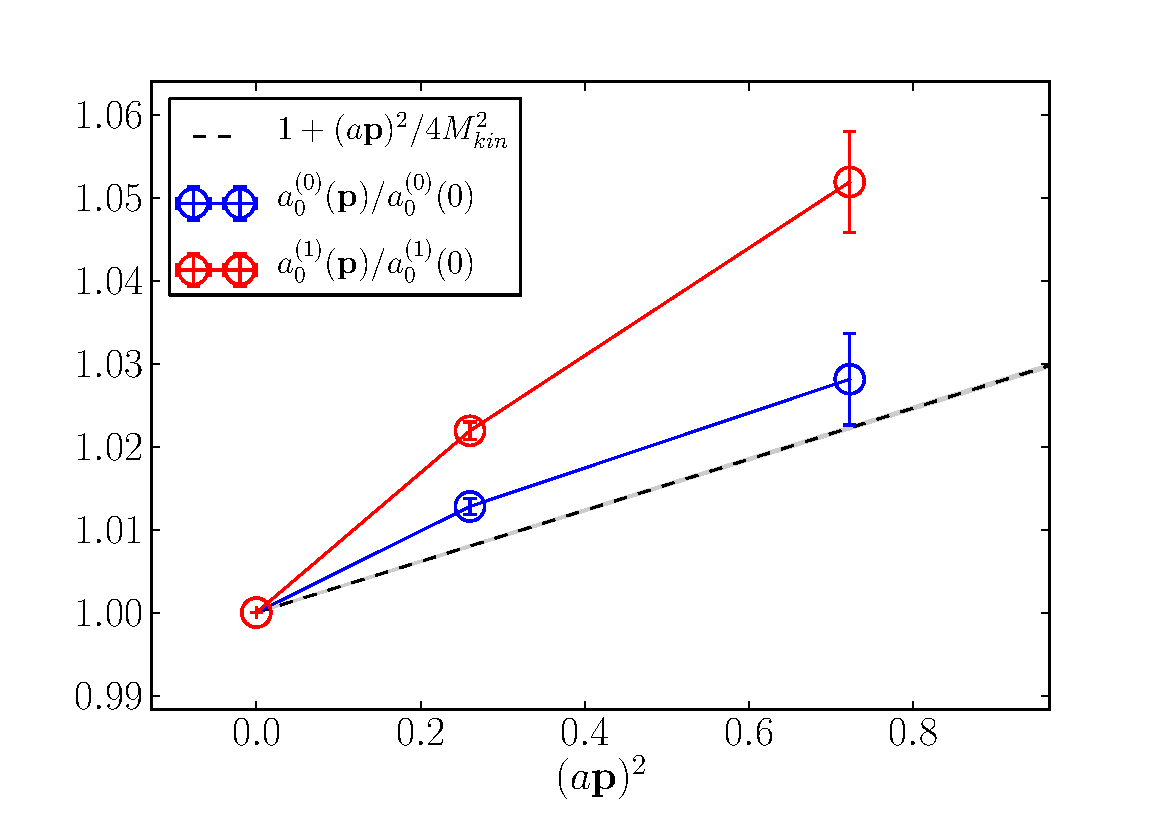
\includegraphics[width=0.85\textwidth]{images/NRQCD/new/relativistic_normalization_J0J1.pdf}
  \end{center}
  \caption{Decay amplitude ratios (colourful points) against the expected relativistic behaviour (grey dotted line and band). Adding the $A_{0,\text{lat}}^{(1)}$ piece of the current does not improve the relativistic behaviour of the ratio. \label{fig:relativisticnorm}}
\end{figure}

%% \subsubsection{Operator Matching}

%% In \cite{Morningstar:1997ep}, it is shown that this operator for the axial current by itself on the lattice is not totally sufficient to represent a continuum axial current. 
%% In this paper, the axial vector current with 1-loop corrections in continuum QCD (illustrated in figure 1, 2 and 3 in \cite{Morningstar:1997ep}) was computed using the on-shell mass and wave function renormalisation scheme in Feynman gauge. The light quark on-shell mass was approximated to zero, and the result was expanded in powers of the inverse heavy quark on-shell mass $1/M$.
%% \begin{align}
%% 	\nonumber
%% 	\langle q(p') | A_0 | h(p) \rangle_{\text{QCD}} = & \eta_1 [ \bar{u}_q(p') \gamma_5\gamma_0 u_h(p) ] + \eta_2 \left[ {p_0\over M} \bar{u}_h(p') \gamma_5 u_h(p) \right] \\
%% 	\nonumber
%% 	+ & \eta_3\left[ {p\cdot p'\over M^2} \bar{u}_q (p') \gamma_5\gamma_0 u_h(p)\right]
%% 	 + \eta_4\left[{p_0'\over M} \bar{u}_q(p') \gamma_5 u_h(p)\right] \\
%% 	 + & \mathcal{O}\left({1\over M^3}\right) \\ \nonumber \\
%% 	 \nonumber
%% 	 \eta_1 =  1 + &{\alpha_s\over 3\pi}\left[ 3\ln {M\over \lambda} - {11\over4} \right] \quad,\quad \eta_2 = {\alpha_s\over 3\pi} 2 \\
%% 	 \nonumber
%% 	 \eta_3 = {\alpha_s\over 3\pi} &\left[ 6\ln {M\over\lambda} - {8\pi\over 3}{M\over\lambda} + {1\over 2} \right] \quad,\quad \eta_4 = {\alpha_s\over 3\pi} \left[ -2 \ln {M\over \lambda} + {1\over 2} \right]
%% 	 \label{eq:continuum_axial}
%% \end{align}
%% $\lambda$ is the artificial Gluon mass (should cancel in obeservables), $|q(p')\rangle$ and $|h(p)\rangle$ are asymptotic light and heavy quark states respectively, and $u_{q,h}$ are the corresponding fermion wavefunctions. 

%% The dimensional requirements that $1/M$ must always come with a power of momenta turns this $1/M$ expansion into an expansion in velocity $v$, so is an NRQCD expansion. There are two expansions at play: $v$ and $\alpha_s$, one should avoid mixing them up.

%% In our lattice simulation the heavy quark obeys NRQCD so only has 2 components (there is no antiparticle without a relativistic dispersion relation). The particle and antiparticle fields in $h(x)$ can be decoupled using the Fouldy-Wouthuysen (FW) transformation \cite{Foldy:1949wa}, which is a canonical transformation, i.e. a change of variables of $h(x)$'s spinor degrees of freedom. Using the FW transformation, one can relate the $u_h$ to the wavefunction of a 2 component quark $U_h(p)$:
%% \begin{align}
%% 	u_h(p) = \exp\left(-{\underline{\gamma}\cdot{\textbf{p}}\over 2M}\right) \binom{U_h(p)}{0}
%% %	\label{eq:FW}
%% \end{align}
%% Using this to replace $u_h$ with $U_h$ in \eqref{eq:continuum_axial}, and inspecting the form of the leading order contributions, one can identify operators in the lattice theory that should be used to reproduce the continuum axial current $A_0$ \cite{Dowdall:2013tga}:
%% \begin{align}
%% 	&A_0 = (1+z_0 \alpha_s ) \left[ A_{0,\text{lat}}^{(0)} + (1 + z_1\alpha_s) A_{0,\text{lat}}^{(1)} + z_2\alpha_s A_{0,\text{lat}}^{(2)} \right]
%% 	\label{eq:current_corrections}
%% \\	&A_{0,\text{lat}}^{(0)} = \bar{c} \gamma_5 \gamma_0 b
%% 	\nonumber
%% \\	&A_{0,\text{lat}}^{(1)} = -{1\over2m_b} \bar{c} \gamma_5 \gamma_0 \underline{\gamma}\cdot\underline{\nabla} b
%% 	\nonumber
%% \\	&A_{0,\text{lat}}^{(2)} = -{1\over2m_b} \bar{c} \underline{\gamma}\cdot\underline{\overleftarrow{\nabla}} \gamma_5 \gamma_0  b.
%% 	\nonumber
%% \end{align}
%% $c$ and $b$ are the quark creation operators. The mass $M$ has been replaced with the bare $b$ mass $m_b$, since the on-shell mass only exists in perturbation theory so has no meaning in terms of the lattice. 
%% The coefficients $\{z_i\}$ can be obtained from matching terms between continuum and lattice perturbation theory.

%% The values $\{z\}$ are not yet known for the $bc$ current, but to give an idea of order or magnitude, in fig. \ref{fig:relativistic} uses values from the temporal axial current between light and $b$ quarks. Taken from \cite{Dowdall:2013tga}, these are $z_0=-0.007(2)$, $z_1=-0.031(4)$, $z_2=-0.325(4)$. $\alpha_s = 0.267$ is taken from set 7 of \cite{Colquhoun:2015oha}, obtained from running down of $\alpha_s^{\overline{MS}}(M_Z)$ down to scales of the simulation dictated by $a$.

%% $A_{0,\text{lat}}^{(0)}$ is the naive current operator used before (i.e with local smearing $\tilde{B}_c = A_{0,\text{lat}}^{(0)}$ in \eqref{eq:correlator}). 
%% To calculate the corrections, 
%% this was replaced with $A_{0,\text{lat}}^{(1,2)}$, and the calculation and fitting was repeated to extract $a_0$, this time coenciding with 
%% $\langle 0 | A_{0,\text{lat}}^{(1,2)} | B_c({\textbf{p}}) \rangle$. From these values one can build up a better estimation to the continuum current 
%% $\langle 0 | A_0 | B_c({\textbf{p}}) \rangle$. In fig. \ref{fig:relativistic} we gradually add corrections to see the effect each has, defining
%% \begin{align}
%%   \nonumber
%%   \label{eq:a_0corrections}
%%   &a_0^{(0)} = \langle 0 | (1+z_0 \alpha_s ) A_{0,\text{lat}}^{(0)} | B_c({\textbf{p}}) \rangle \\
%%   &a_0^{(1)} = \langle 0 | (1+z_0 \alpha_s ) \left[ A_{0,\text{lat}}^{(0)} + (1 + z_1\alpha_s) A_{0,\text{lat}}^{(1)} \right] | B_c({\textbf{p}}) \rangle \\
%%   \nonumber
%%   &a_0^{(2)} = \langle 0 | (1+z_0 \alpha_s ) \left[ A_{0,\text{lat}}^{(0)} + (1 + z_1\alpha_s) A_{0,\text{lat}}^{(1)} + z_2\alpha_s A_{0,\text{lat}}^{(2)} \right] | B_c({\textbf{p}}) \rangle \\
%%   \nonumber
%% \end{align}

%% \begin{table}
%% \begin{center}
%%  \begin{tabular}{||c c c c c c c c c||} 
%%  \hline
%%  set & $(a{\textbf{p}})^2$ & $a\delta E_0({\textbf{p}})$  & $aM_{B_c}$ & $a_0^{(0)}({\textbf{p}})/a_0^{(0)}(0)$ & $a_0^{(1)}({\textbf{p}})/a_0^{(1)}(0)$ 
%%  & $a_0^{(2)}({\textbf{p}})/a_0^{(2)}(0)$ \\ [0.5ex] 
%%  \hline\hline
%%  1 & 0.02891 & 0.00537(23) & 2.61(11) & 1.0036(19) & 1.0046(21) & 1.0045(21) \\ \hline
%%  2 & 0.26023 & 0.04580(24) & 2.838(27) & 1.0164(23) & 1.0253(26) & 1.0251(26) \\ \hline
%%  3 & 0.72287 & 0.12456(46) & 2.823(14) & 1.0371(46) & 1.0615(50) & 1.0608(51) \\ \hline
%%  4 & 1.04093 & 0.17772(86) & 2.840(15) & 1.053(10) & 1.088(11) & 1.086(11) \\ [1ex] 
%%  \hline
%% \end{tabular}
%% \end{center}
%% \caption{Results from fits with varying momenta. The third column gives the kinetic mass deduced from $\delta E({\textbf{p}})$ for each ${\textbf{p}}$. using \eqref{eq:kinetic_mass}\label{tab:from_fit}}
%% \end{table}

%% \subsubsection{$A_0^{(3)}$ contribution}

%% These current corrections are only to $\mathcal{O}({\textbf{p}}_b/m_b)$, but $\sqrt{E^r_{B_c}/M_{B_c}}$ has it's leading behaviour in $\mathcal{O}({\textbf{p}}^2/M_{B_c}^2)$. This implies one needs to carry on the expansion of current corrections further, to $\mathcal{O}(1/m_b^2)$. The dominant term at this order arises at tree level from the first term in \eqref{eq:continuum_axial}, and the second term in a $1/M$ expansion of \eqref{eq:FW}. The corresponding lattice operator is
%% \begin{align}
%% 	A^{(3)}_{0,\text{lat}} = {1\over 8m_b^2} \bar{c} \gamma_5\gamma_0 \underline{\nabla}^2 b. 
%% \end{align}
%% This was computed in a lattice calculation and combined with the lower orders to produce $a^{(3)}_0 = a_0^{(2)} + A^{(3)}_{0,\text{lat}}$. In this case we set $\alpha_s = 0$ to just focus on tree level. The results are shown on fig. \ref{fig:A3}.
%% \begin{figure}
%% \begin{center}
%%     \begin{tikzpicture}
%%         \begin{axis} [width=14cm,height=9cm,
%%             xmin=-0.1,xmax=0.9,ymin=0.99,ymax=1.09,
%%             xlabel = $(a{\textbf{p}})^2$,
%%             legend pos=north west]

%%             \addplot[color=green, dashed]{ sqrt( sqrt( x + 2.834*2.834 )/2.834) };
%%             \addlegendentry{$\sqrt{E_{B_c}/M_{B_c}}$}

%%             \addplot+[color=blue, mark=*,
%%                     error bars/.cd,x dir=both, x explicit,  y dir=both, y explicit]
%%                 coordinates {
%%                 		(  0.0 ,  1.0  ) +- ( 0.0,  1.33226762955e-19  )
%% 		  	(  0.0289148446127 ,  1.00549267643  ) +- ( 0.0,  0.00176452228481  )
%% 			(  0.260233601514 ,  1.01836440302  ) +- ( 0.0,  0.00222088535291  )
%% 			(  0.722871115317 ,  1.0390590324  ) +- ( 0.0,  0.00452197676768  )
%%             };
%%             \addlegendentry{$a_0^{(0)}({\textbf{p}})/a_0^{(0)}(0)$}

%%             \addplot+[color=red, mark=*,
%%                     error bars/.cd,x dir=both, x explicit,  y dir=both, y explicit]
%%                 coordinates {
%%                 		(  0.0 ,  1.0  ) +- ( 0.0,  0.0  )
%%           	        (  0.0289148446127 ,  1.00663334793  ) +- ( 0.0,  0.00194538583335  )
%% 			(  0.260233601514 ,  1.02734203998  ) +- ( 0.0,  0.00244820981549  )
%% 			(  0.722871115317 ,  1.06347584999  ) +- ( 0.0,  0.00497690081001  )
%%             };
%%             \addlegendentry{$a_0^{(1)}({\textbf{p}})/a_0^{(1)}(0)$}
            
%%             \addplot+[color=orange, mark=*,
%%                     error bars/.cd,x dir=both, x explicit,  y dir=both, y explicit]
%%                 coordinates {
%%                 		(  0.0 ,  1.0  ) +- ( 0.0,  0.0  )
%% 			(  0.260233601514 ,  1.0211157939  ) +- ( 0.0,  0.00302333986783  )
%% 			(  0.722871115317 ,  1.05858288737  ) +- ( 0.0,  0.00568371480017  )
%%             };
%%             \addlegendentry{$a_0^{(3)}({\textbf{p}})/a_0^{(3)}(0)$}

%%         \end{axis}
%%     \end{tikzpicture}
%% \end{center}
%% \caption{Relativistic Normalisation of 1-loop corrected Axial Current. $a_0^{(n)}$ are defined in \eqref{eq:a_0corrections}. (tree level) }
%% \label{fig:A3}
%% \end{figure}
%% As a sanity check for the $A^{(3)}$ calculation, fig. \ref{fig:A3A2} shows the ratio $A^{(3)}_{0,\text{lat}}({\textbf{p}})/A^{(2,1)}_{0,\text{lat}}({\textbf{p}})$. Since $A^{(3)} = \mathcal{O}({\textbf{p}}^2)$ and $A^{(1)} = \mathcal{O}({\textbf{p}})$, we expect such a ratio to be proportional to $|{\textbf{p}}|$ (see fig. \ref{fig:A3A1}). {\color{red}{The $A^{(3)}/A^{(2)}$ line isn't straight...}}

%% %==========
%% \begin{figure}
%% \begin{center}
%%     \begin{tikzpicture}
%%         \begin{axis} [width=14cm,height=9cm,
%%             xlabel = $a|{\textbf{p}}|$,
%%             legend pos=north west]

%%             \addplot+[color=red, mark=*,
%%                     error bars/.cd,x dir=both, x explicit,  y dir=both, y explicit]
%%                 coordinates {
%%                		(  0.0 ,  0.168061897514  ) +- ( 0.0,  0.00761364082979  )
%% 			(  0.510130965061 ,  0.255812358549  ) +- ( 0.0,  0.0171547894616  )
%% 			(  0.850218275102 ,  0.291882276843  ) +- ( 0.0,  0.0323767757253  )
                    
%%             };
%% \addlegendentry{$A^{(3)}_{0,\text{lat}}({\textbf{p}})/A^{(1)}_{0,\text{lat}}({\textbf{p}})$}

%%         \end{axis}
%%     \end{tikzpicture}
%% \end{center}
%% \label{fig:A3A1}
%% \caption{Ratio of third current correction to first.}
%% \end{figure} 

\section{$B_{(s)}\to D_{(s)}l\nu$ form factors}
\label{sec:BD_BsDs_nrqcd}

We attempted a calculation of the $B\to Dl\nu$ and $B_{s}\to D_{s}l\nu$ form factors, $f_{0,+}(q^2)$ and $f^s_{0,+}(q^2)$, using the 2+1+1 MILC ensembles, HISQ $l$,$s$ and $c$ valence quarks, and an NRQCD valence $b$ quark. This study was similar to previous studies of $B\to Dl\nu$ form factors \cite{Na:2015kha} and $B_s\to D_sl\nu$ form factors \cite{Monahan:2017uby}. The main difference between this study and the previous studies was that they used older MILC ensembles not taking the charm into account in the sea.

\subsection{Calculation Details}

\begin{table}[htb!]
\hspace{-40pt}
 \begin{tabular}{c c c c c c c c c c c}
 \hline
 Set & handle & $am_{s0}$ & $am_{c0}$ & $am_{b0}$ & $u_0$ & $c_{1,6}$ & $c_5$ & $c_4$ & $\{T\}$ & $a_{\text{sm}}/a$ \\ [0.5ex] 
 \hline
 0 & {\textbf{very coarse}} & 0.0705 & 0.826 & 3.297 & 0.8195 & 1.36 & 1.21 & 1.22 & 8, 11, 14 & 0, 2.0, 4.0 \\ [1ex]
 1 & {\textbf{coarse}} & 0.0541 & 0.645 & 2.66 & 0.8340 & 1.31 & 1.16 & 1.20 & 9, 12, 15 & 0, 2.0, 4.0 \\ [1ex]
 2 & {\textbf{fine}} & 0.0376 & 0.450 & 1.91 & 0.8525 &  1.21 & 1.12 & 1.16 & 14, 19, 24 & 0, 3.425, 6.85 \\ [1ex]
 \hline
\end{tabular}
 \caption{Parameters used in our calculation. $am_{s0}$ and $am_{c0}$ are the bare masses of the strange, charm valence quarks, tuned in \cite{PhysRevD.91.054508}, $am_{b0}$ is the bare mass of the valence bottom quark, tuned in \cite{Dowdall:2011wh} $u_0$ is the 'tadpole improvement parameter' as used in \cite{Dowdall:2011wh}. $\{c_i\}$ are the coefficients for the kinetic and chromomagnetic terms in the NRQCD action (eq. \eqref{eq:nrqcd_dH}) \cite{Hammant:2013sca}. $\{T\}$ is the set of temporal seperations between source ($B_s$ creation operator) and sink ($D_s$ anihilation operator). $a_{\text{sm}}$ are the radii of the exponential smearing function applied to the $B_{(s)}$ and $D_{(s)}$ creation operators.
   \label{tab:quarkmasses}}
\end{table}

We generated correlation functions on three MILC ensembles, sets 0, 1 and 2 in table \ref{tab:ensembles}. When using the NRQCD action, we are limited to the coarser end of the spectrum of ensembles, since in the $a\to 0$ limit subleading terms in $\delta H$ (eq. \eqref{eq:nrqcd_dH}) and $J^{(n>0)}_{\mu}$ (eq. \eqref{eq:nrqcd-hisq-current}) diverge. However, NRQCD discretisation effects are small relative to other discretizations due to the lack of the $b$ rest mass, so we can afford to use coarser lattices. Also, obviously, using coarse lattices means the project is computationally inexpensive. The bare parameters used to generate the correlation functions are shown in table \ref{tab:quarkmasses}.

We generate 2-point correlation functions for $B_{(s)}$ and $D_{(s)}$ mesons, and 3-point correlators between $B_{(s)}$ and $D_{(s)}$ creation/anihilation operators with $V^{(n)}_{\mu}$ currents inserted for all $\mu$ and $n=0,1,2,3,4$. For the $B_{(s)}$ operator we use smearings like those introduced in eq. \eqref{eq:smearings}, smearing radii $a_{\text{sm}}$ are given in table \ref{tab:quarkmasses}.

The $B_{(s)}$ 2-point correlators, $C_{D_{(s)}}^{\alpha\beta}(t)$ are generated using eq. \eqref{eq:nrqcd-hisq-2pt}, with the charm propagator replaced with a strange or light propagator, and $\mathcal{O}_{m} = \gamma_0\gamma_5$. We generate $D_{(s)}$ 2-point correlators at a number of spacial momenta $\{{\textbf{p}}\}$, generated by
\begin{align}
  C_{D_{(s)}}^{\alpha\beta}({\textbf{p}},t) = \sum_{\textbf{x},\textbf{y}} \phi^{\alpha}({\textbf{x}})\phi^{\beta}({\textbf{y}}) \text{Tr}_c[g_c^{\theta}(x,y) g^{\dagger}_{l(s)}(x,y) ].
\end{align}
where $\phi^{\alpha}({\textbf{x}})$ are the smearing functions defined in eq. \eqref{eq:smearings}, $g_{l(s)}$ are light or strange staggered propagators, and $g_c^{\theta}$ is a charm staggered propagator with momentum twist $\theta$. Tr$_c$ is over color.

We generate 3-point correlators for each individual piece of the NRQCD-HISQ currents, and each chosen $D_{(s)}$ spacial momentum, using
\begin{align}
  C_{V_{\mu}^{(n)}}^{\alpha\beta} ({\textbf{p}},t,T) = \sum_{\textbf{x},\textbf{y},\textbf{z}} \text{Tr}_c\left( g_c^{\theta}(x,y) g_{l(s)}^{\dagger}(x,z) \text{Tr}_s\left[ \gamma_0 \gamma_x\gamma_y \mathcal{O}_{n,\mu}G_b(y,z) \gamma_z \right] \right).
\end{align}
The list of twists we ran on each ensemble is given in table \ref{tab:nrqcd_twists}. Due to the signal/noise degredation of the $D_{(s)}$ correlators as one adds more spacial momentum, our lattice data was limited to the high $q^2$ region. One motivation for this study was to test how far down the $q^2$ range we could reach with lattice data before the noise in the correlators made the data useless.

\begin{table}[htb!]
\begin{center}
 \begin{tabular}{c c c c c}
 \hline
 & Set & $\theta$ & $|a{\textbf{p}}|$ & $q^2$[GeV$^2$] \\ [0.5ex] 
 \hline
 $B\to D$ & 0 & 0, 0.74, 1.47, 2.20, 2.94 & 0, 0.25, 0.5, 0.75, 1.00 & \\ [1ex]
 & 1 & 0, 1.58, 2.24, 4.53 & 0, 0.36, 0.51, , 1.02 & \\ [1ex]
 & 2 & 0, 1.76, 2.64 & 0, 0.30, 0.49 \\ [1ex]
 \hline
 $B_s\to D_s$ & 0 & 0, 0.74, 1.47, 2.20, 2.94 & 0, 0.25, 0.5, 0.75, 1.03 & \\ [1ex]
 & 1 & 0, 1.10, 2.20, 3.31, 4.41 & 0, 0.25, 0.50, 0.75, 1.00 & \\ [1ex]
 & 2 & 0 & 0 & \\ [1ex]
 \hline
\end{tabular}
 \caption{Twists given to the charm propagator on each ensemble. \label{tab:nrqcd_twists} }
 \end{center}
\end{table}

{\red{
    =============================
    
    Have written up to here, everything below is old!

    =============================}}


%\\ \\
%\\ \\
Table \ref{tab:nrqcdensembles} gives details of the ensembles used in this study. These are taken from the MILC HISQ ensembles \cite{Bazavov:2012xda}. They are generated by MCMC with the distribution given in \eqref{eq:MCweight}, where $M$ is the Dirac operator for the HISQ action. They take into accound up, down, strange and charm quarks, assuming the contribution from higher mass quarks in the sea to be negligable.
\\ \\
Following the procedure discussed in section \ref{sec:correlators}, first we must compute 2-point correlators for the $B_s$ and $D_s$. In both cases we use \textit{smeared} creation operators:
\begin{align}
	\Phi^{\alpha}(\underline{k},t) = \sum_{\underline{x},\underline{x'}} e^{-i\underline{k}\cdot\underline{x}} \text{ } \bar{\psi}_1(\underline{x'},t)\phi^{\alpha}(\underline{x}'-\underline{x}) \gamma_5 \psi_2(\underline{x})
\end{align}
where $\bar{\psi}_1$,$\psi_2$ are $\bar{b}$,$s$ for the $B_s$ and $\bar{c}$,$s$ for the $D_s$. The smearing functions $\phi^{\alpha}$ approximate the wavefunction of one quark in a potential set up by the other, giving a psuedo-realistic representation of the meson. This makes the operator $\Phi^{\alpha}$ couple stronger to the ground state of the meson, maximizing the $a_0 \propto \langle0 |\Phi^{\alpha}|\lambda_0\rangle$ parameter in the fit \eqref{eq:multiexponential} relative to the excited states $a_{n>0}$. This increases the dominance of the first term in \eqref{eq:multiexponential} resulting in better convergence of the $n$ sum, therefore a better fit and better statistics of the results.
\\ \\
For the $B_s$, we use a combination of $\phi^0(\underline{z})=\delta(\underline{z})$ ("local"), and $\phi^{1,2}(\underline{z}) \propto \text{exp}(-|\underline{z}|/r_0)$ ("smeared"), with $r_0 \simeq 2.5$fm$, 5$fm. For the $D_s$ we use one local and one smeared with $r_0\simeq2.5$fm. Correlation functions between each smearing combination is calculated, i.e. for the $D_s$, we compute 4 correlators $\langle \Phi^{0\dagger}_D\Phi_D^0 \rangle$, $\langle \Phi^{1\dagger}_D\Phi_D^0 \rangle$, $\langle \Phi^{0\dagger}_D\Phi_D^1 \rangle$, $\langle \Phi^{1\dagger}_D\Phi_D^1 \rangle$, and 9 for the $B_s$.
\\ \\
A good way to see the benefit of the smearing is by plotting the effective mass $m_{\text{eff}}(t) = \text{log}({C(t)/C(t+1)})$ against $t$ as in fig. \ref{fig:effmass}. The flatness of this as a function in $t$ shows how well it is approximated by the fit function with only the ground state (i.e. not contaminated by excited states), therefore how easily the fit will determine the ground-state energy. As can be seen, The smeared effective mass "flattens out" quicker than the local, as the smeared couples mostly to the ground state.
\\ \\
\begin{figure}
  \begin{center}
    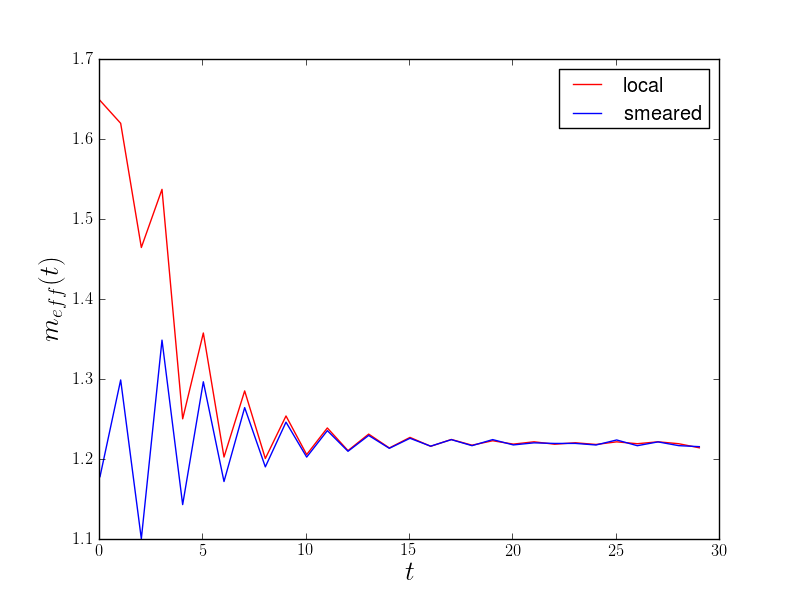
\includegraphics[width=0.65\textwidth]{images/NRQCD/EffMass_localVsSmear_Ds_coarse.png}
  \end{center}
  \caption{Effective mass of $D_s$ correlation functions, one with local $D_s$ operators $\langle\Phi^0\Phi^0\rangle$ and one with smeared $\langle\Phi^1\Phi^1\rangle$.}
  \label{fig:effmass}
\end{figure}

The 3pt correlation function calculated is $\langle \Phi^{\alpha\dagger}_{D_s} V_{\mu} \Phi^{\beta}_{B_s} \rangle$, including all smearings of the $B_s$ and $D_s$ used in the 2-point functions. We must be careful choosing the appropriate operator for $V_{\mu}$. Recall that NRQCD quarks contain an inverse Fouldy-Wouthuysen (FW) transformation \eqref{eq:FoldyWoldy}. This must be encorparated into the $V_{\mu}$ operator, since it couples to the $b$ which obeys the NRQCD action in our simulation. Hence the $V_{\mu}$ operator must be of the form
\begin{align}
	V_{\mu} = \bar{c}\gamma_{\mu}\left( 1 - {1\over 2m_b} \underline{\gamma}\cdot\underline{\nabla} + \mathcal{O}\left({1\over m_b^2}\right) \right) b 
\end{align}
where we can afford to expand the exponential in the FW transformation since $1/m_b$ is small. However, this is only a tree level result. According to the discussion in sec. \ref{sec:renormalization}, these terms require renormalization constants, and also new terms in the above expansion may appear. Therefore the full expression for the vector current that we use is (accurate to $\mathcal{O}(\alpha_s,1/m_b)$):
\begin{align}
	\nonumber
	V_{\mu} &= (1+z_0 \alpha_s)\left[ V_{\mu}^{(0)} + (1 + z_1 \alpha_s) V_{\mu}^{(1)} + z_2 \alpha_s V_{\mu}^{(2)} \right] \\
	\nonumber
	& V_{\mu}^{(0)} = \bar{c}\gamma_{\mu} b \\
	\nonumber
	& V_{\mu}^{(1)} = -{1\over 2m_b} \bar{c} \gamma_{\mu}\underline{\gamma}\cdot\underline{\nabla} b \\
	\nonumber
	& V_{\mu}^{(2)} = -{1\over 2m_b} \bar{c} \gamma_{\mu}\underline{\gamma}\cdot\underline{\overleftarrow{\nabla}} b \\
	\label{eq:currentcorrections}
\end{align}
The coefficients $\{z_i\}$ are set by a matching procedure between the HISQ/NRQCD currents and continuum QCD in \cite{Monahan:2012dq}. We calculate correlation functions $\langle \Phi_{D_s} V^{(i)}_{\mu} \Phi_{B_s}\rangle$ for each current and combine them after the fitting procedure.

\subsection{Deduction of Form Factors}

We wish to use these currents to deduce the $B_s\to D_s l\nu$ form factors discussed in section \ref{sec:formfactors} over the full $q^2$ range. To this end, the above procedure to compute $\langle D_s | V^{(i)}_{\mu} | B_s \rangle$ is repeated while giving the $D_s$ meson a range of different spacial momenta. We chose spacial momentum ${\textbf{p}} = |{\textbf{p}}|(1,1,1)$, in this each direction is equivilant, and it allows us to average $V_{\mu}$ over the 3 spacial directions, reducing work in the fit and increasing the statistics of the averaged current $V_k \equiv \sum_{i=1}^3 V_i / 3$.
\\ \\
As discussed in appendix \ref{sec:signalnoise}, the most accurate results will come from $|{\textbf{p}}| = 0$, then the correlators become noise-dominated as one increases $|{\textbf{p}}|$ towards $|{\textbf{p}}|_{\text{max}}$. Hence, the approach is to start at the $|{\textbf{p}}|=0$ end and move up in momentum, monitoring statistical errors as you go. So far we have performed runs for $|a{\textbf{p}}| = 0,0.30,0.45$ on the fine ensemble, and $|a{\textbf{p}}|=0,0.25,0.50$ on the coarse ensemble. Statistical errors have not yet become uncontrollable at these momenta, but from experience of previous calculations, they are expected to become problematic at $|a{\textbf{p}}| \sim 0.7$. 
\\ \\
With values for $\langle D_s | V_{\mu} | B_s \rangle$ at varying ${\textbf{p}}$ therefore varying $q^2$, we can perform a fit of this data in order to extract $f_{0,+}(q^2)$ via \eqref{eq:formfactors}. To do the fit, we need some anzats for the functional form of $f_{0,+}(q^2)$. We use the BCL parameterization \cite{PhysRevD.79.013008}. This involves first reparameterizing $q^2$ to 
\begin{align}
	z(q^2) = {\sqrt{t_+ - q^2} - \sqrt{t_+ - t_0} \over \sqrt{t_+ - q^2} + \sqrt{t_+ - t_0} }
\end{align}
where we take $t_0 = t_+( 1 - \sqrt{1 - t_-/t_+})$, and $t_{\pm} = (M_{B_s} \pm M_{D_s})^2$, as in \cite{Hill:2006ub}. $z(q^2)$ has a very small magnitude throughout the entire $q^2$ range, in our case $|z|_{\text{max}} \sim 0.032$. We can then accurately model $f_{+,0}$ as a series expansion in $z$:
\begin{align}
	f_{0,+}(q^2) = {1\over P_{0,+}(q^2)} \sum_n a^{0,+}_n z(q^2)^n
	\label{eq:zexpansion}
\end{align}
we truncate this at $z^2$, adding further terms have no effect on the fit. The so-called Blaschke factors $P(q^2)$
are defined by
\begin{align}
	P_{0,+}(q^2) = \left( 1 - {q^2\over M_{0,+}^2}\right)
\end{align}
These are required due to subthreshold poles in the crossed channel of $\langle D_s | V^{(i)}_{\mu} | B_s \rangle$, which in our case is a $W$ decay into a $B_c$ meson. The pole is located where the $W$ has the correct momentum $q^2$ to create the $B_c$, hence at $q^2=M_{B_c}$. This is not within the $q^2$ range, but can create curvature in $f_{0,+}$ that can confound the expansion in $z$. $P_{0,+}$ effectively removes this pole from the $z$ expansion.

\subsection{Continuum \& Chiral Extrapolation}

The form factors $f_{0,+}(q^2)$ we deduce from the above will contain systematic errors due to 1) discretization, and 2) unphysical quark masses and mistunings. 
\\ \\
2) requires a little explaination. In lattice simulations it is computationally expedient (and sometimes neccesary) to take the up/down quark masses $m_l$ to be much larger than their physical values. This is because the condition number of the Dirac operator $M_l$ is proportional to $am_l$, a small condition number makes it difficult or impossible to numerically invert $M_l$ to obtain the propagator $M^{-1}_l$ as part of the process in section \ref{sec:correlators}. Fortunately, since the $B_s\to D_s l\nu$ decay involves no up/down valence quarks, we mostly need not worry about this problem. There is also the issue of mistuning: the quark masses we use are tuned by a calculation of some process, see caption in table \ref{table:quarkmasses}. The uncertainty in these determinations must be accounted for somehow.
\\ \\
The above issues are in general dealt with by computing the above form factors at a number of lattice spacings and quark masses, and results extrapolated to $a\to 0$ and $m\to m_{\text{physical}}$. The $a\to 0$ extrapolation is performed by involving data from all ensembles in the fit to $f_{0,+}$, and modifying \eqref{eq:zexpansion}:
\begin{align}
	a^{0,+}_n \to a^{0,+}_n \times ( 1 + b^{0,+}_n (am_c)^2 )
\end{align}
where $b^{0,+}_n$ are new fit parameters, and $m_c$ is the charm mass. $am_c\to0$ in the continuum limit, and, since the charm mass is the largest mass parameter involved in our calculation, it serves as a good order parameter for discretization effects. The extrapolation in masses has not yet been implemented in this work.

\section{Results I guess}
\label{sec:nrqcd}

%% \begin{figure}
%% \centering
%% \begin{subfigure}{.55\textwidth}
%%   \centering
%%   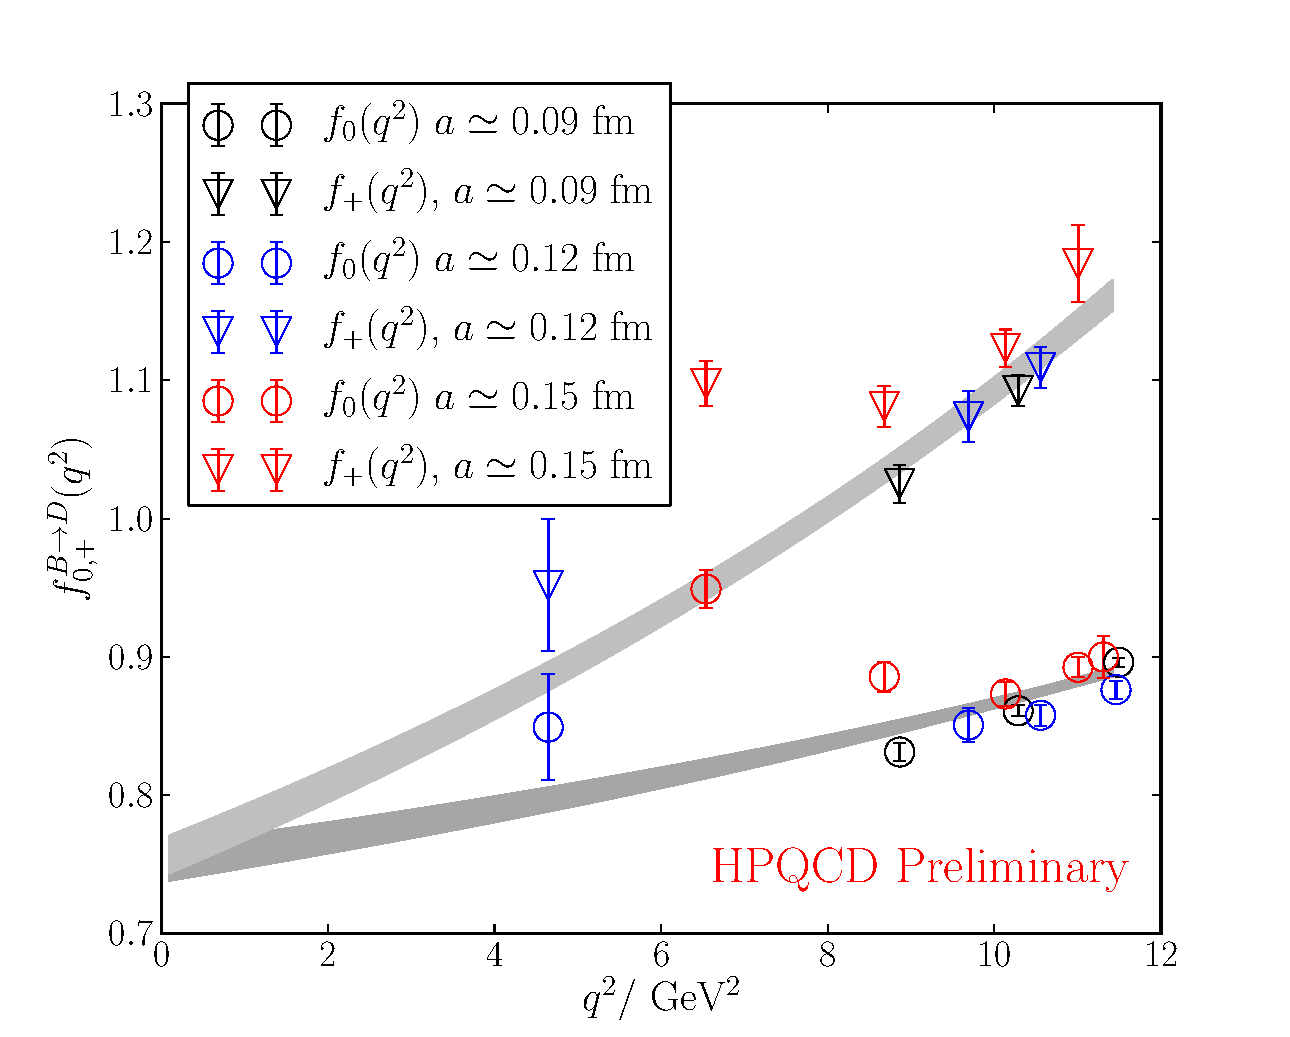
\includegraphics[width=1.0\linewidth]{images/NRQCD/BD_apr18.pdf}
%%   \label{fig:sub1}
%% \end{subfigure}%
%% \begin{subfigure}{.55\textwidth}
%%   \centering
%%   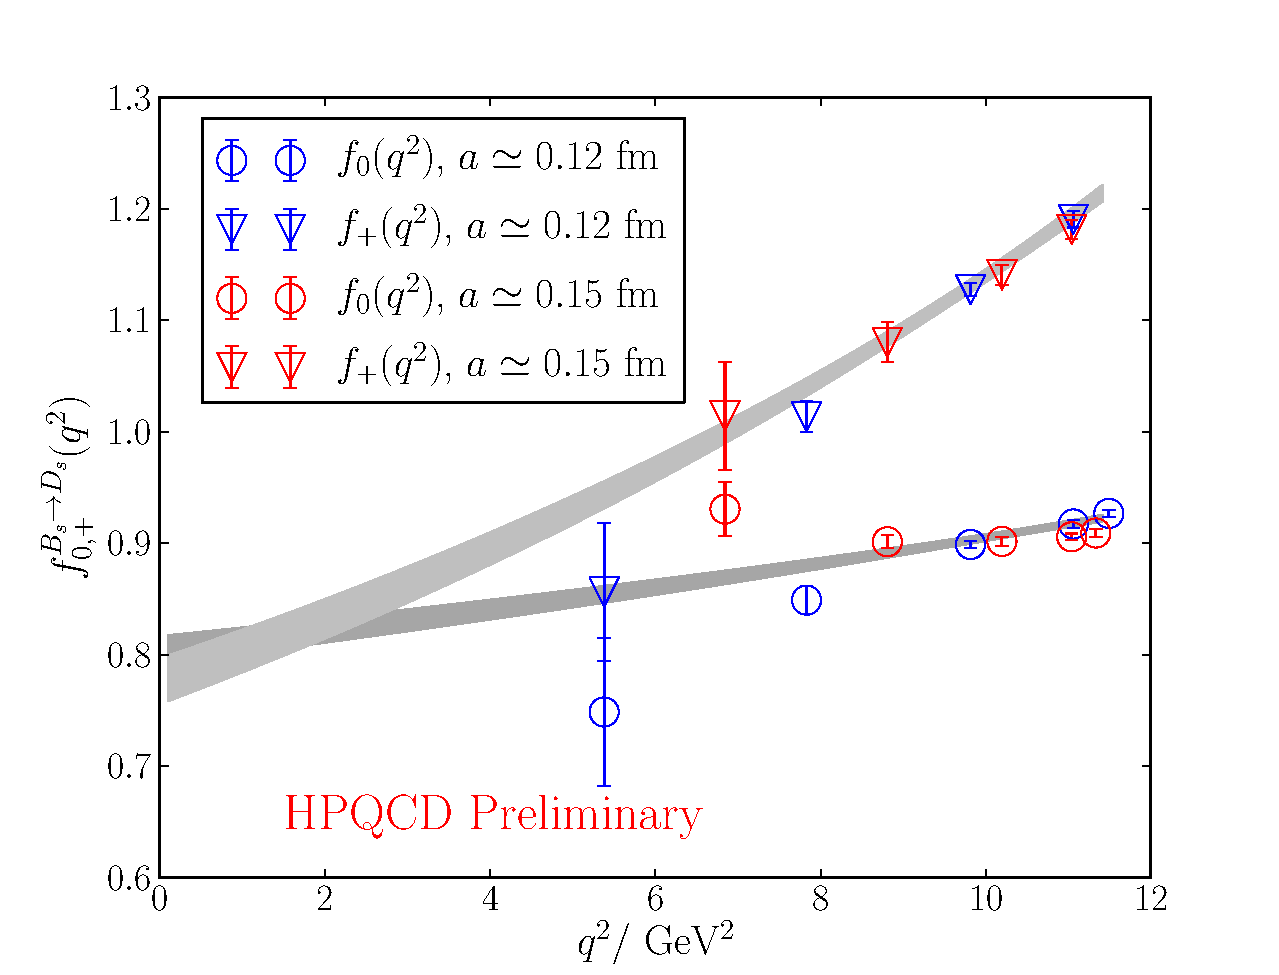
\includegraphics[width=1.0\linewidth]{images/NRQCD/BsDs_apr18.pdf}
%%   \label{fig:sub2}
%% \end{subfigure}
%% \caption{Left: $B\to D l\nu$ form factors from the NRQCD calculation. Right: $B_s\to D_s l\nu$ form factors using an identical approach. Errors are statistical. The bands give a kinematic extrapolation to all $q^2$, see second year report. The statistical errors grow as $q^2$ decreases due to Parisi-Lepage scaling (sec.9.3.2 of \cite{DeGrand:2006zz}).}
%% \label{fig:nrqcd}
%% \end{figure}

\begin{figure}
  \vspace{-20pt}
  \begin{center}
    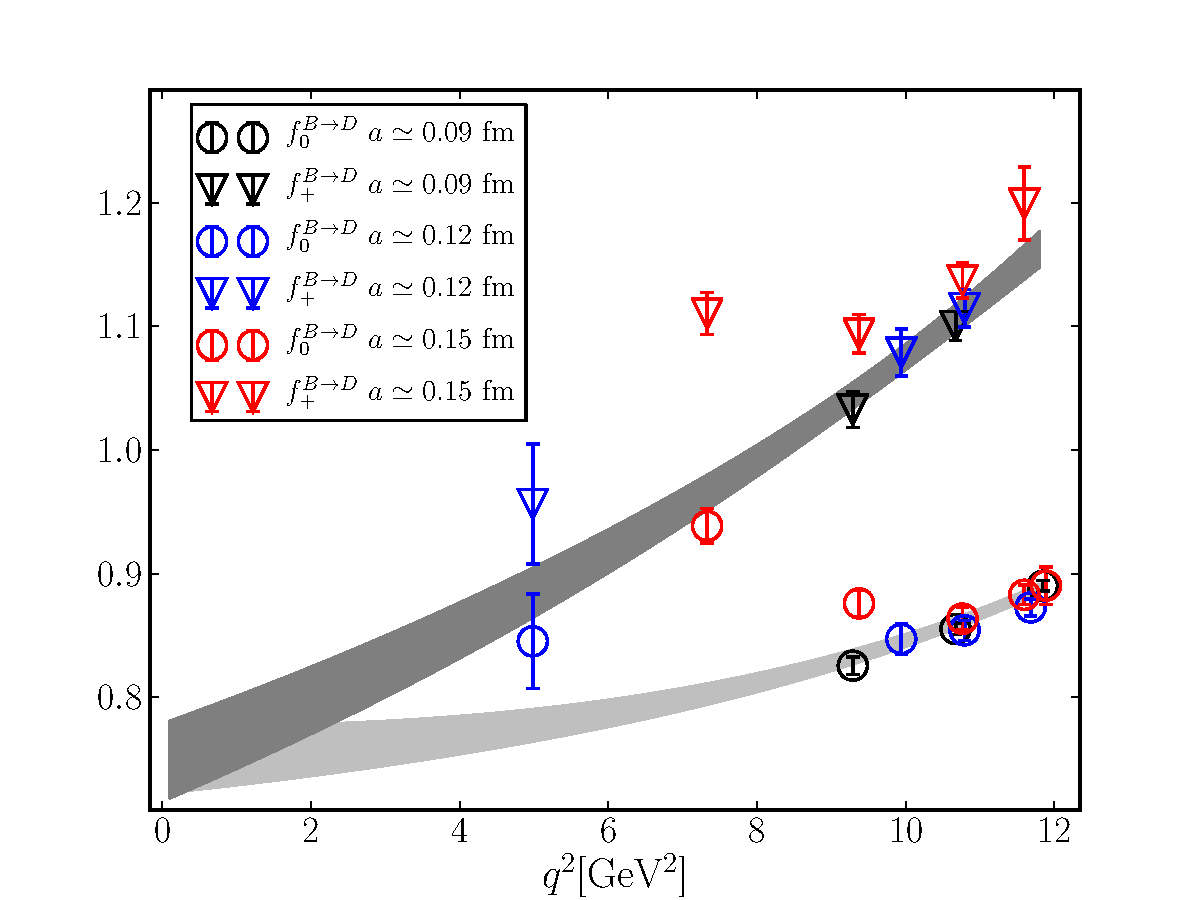
\includegraphics[width=0.85\textwidth]{images/NRQCD/new/BD_formfactors.pdf}
  \end{center}
  \caption{}
  \vspace{-20pt}
\end{figure}

\begin{figure}
  \vspace{-20pt}
  \begin{center}
    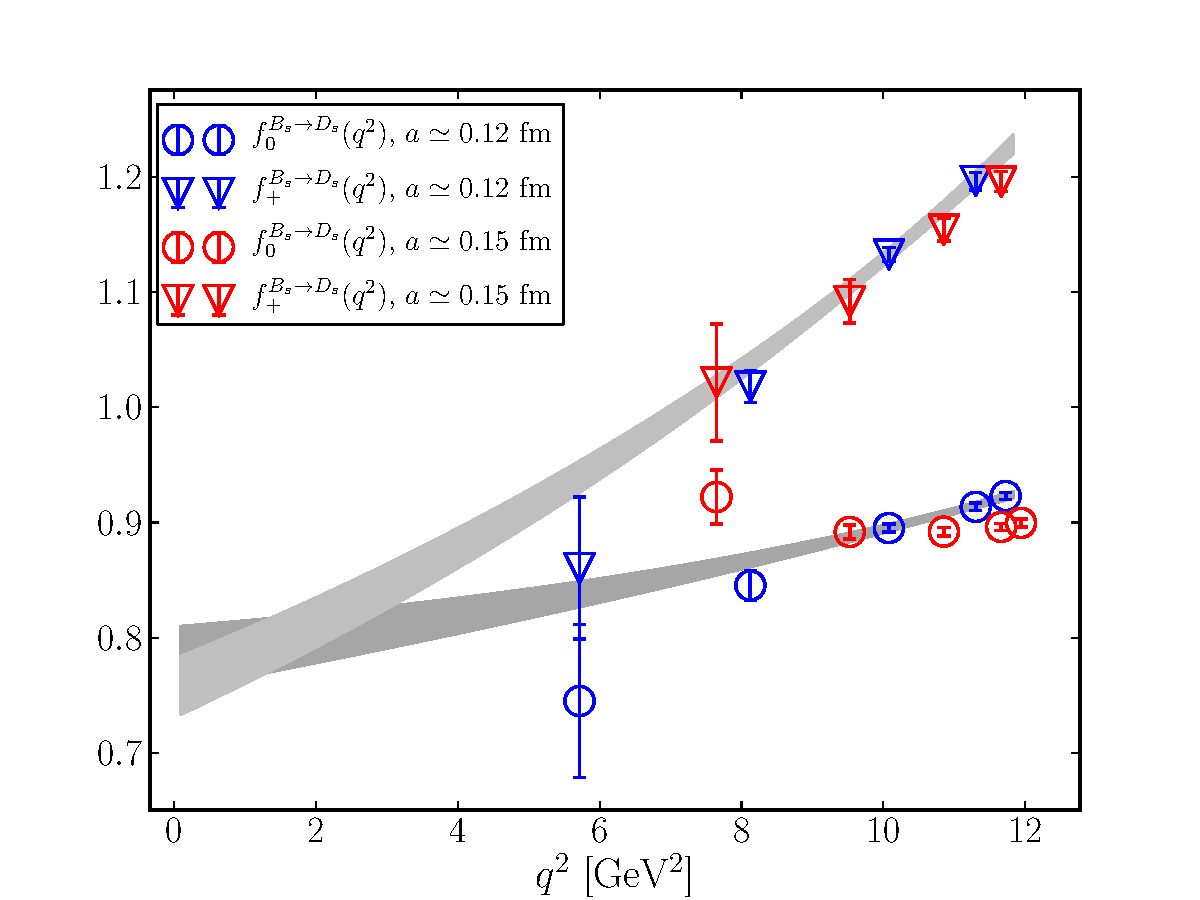
\includegraphics[width=0.85\textwidth]{images/NRQCD/new/BsDs_formfactors.pdf}
  \end{center}
  \caption{}
  \vspace{-20pt}
\end{figure}

\begin{figure}
  \vspace{-20pt}
  \begin{center}
    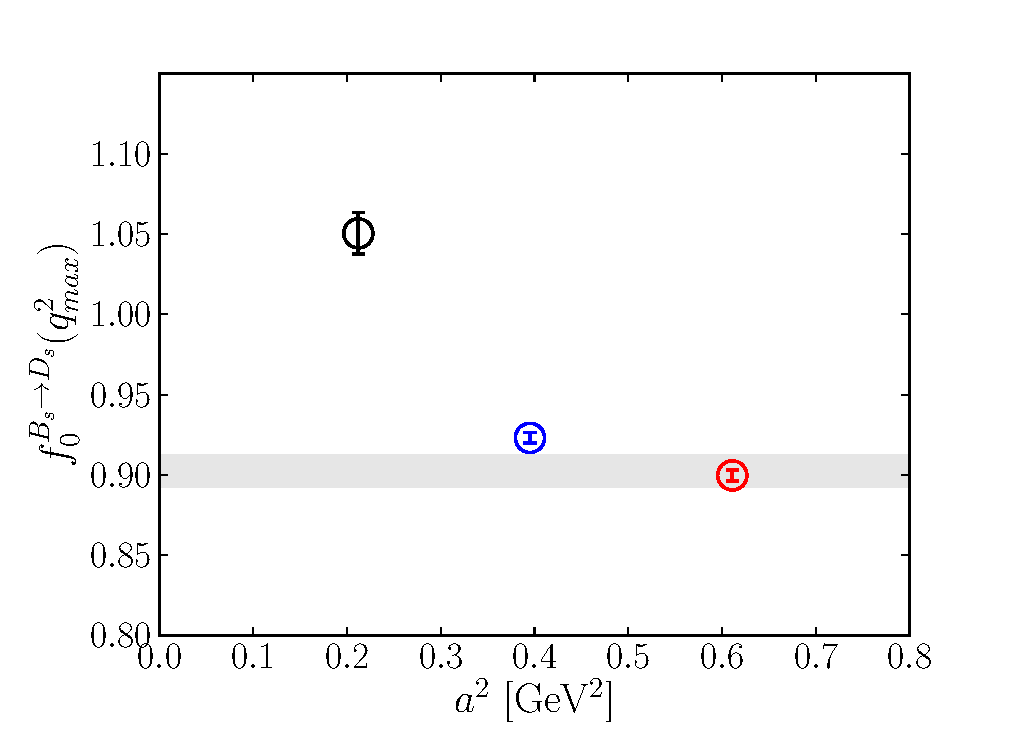
\includegraphics[width=0.75\textwidth]{images/NRQCD/new/BsDs_f0q2max.pdf}
  \end{center}
  \caption{}
  \vspace{-20pt}
\end{figure}


\begin{table}
\begin{center}
\begin{tabular}{|| c c c c c c c c ||}
\hline
Set & $|a{\textbf{p}}_{D_s}|$ & $V_0^{(0)}$ & $V_0^{(1)}$ & $V_0^{(2)}$ & $V_k^{(0)}$ & $V_k^{(1)}$ & $V_k^{(2)}$ \\ [0.5ex]
\hline \hline
2 & 0.00 & 0.3819(12) & 0.0024(12) & 0.0(1.0)e-05 & 0.0(1.0)e-05 & 0.0(1.0)e-05 & 0.0(1.0)e-05\\ [0.5ex] 
 & 0.25 & 0.3726(18) & 0.00281(61) & 0.00109(67) & 0.02317(28) & 0.00057(17) & -0.00572(39)\\ [0.5ex] 
 & 0.50 & 0.3522(18) & 0.00339(53) & -0.00390(75) & 0.04309(51) & 0.00111(42) & -0.01106(57)\\ [0.5ex] 
3 & 0.00 & 0.3719(62) & 0.0048(14) & 0.0(1.0)e-05 & 0.0(1.0)e-05 & 0.0(1.0)e-05 & 0.0(1.0)e-05\\ [0.5ex] 
 & 0.30 & 0.3465(73) & 0.0045(19) & 0.0006(19) & 0.03692(49) & 0.00128(92) & -0.00869(91)\\ [0.5ex] 
 & 0.45 & 0.3426(39) & 0.0052(14) & -0.0054(14) & 0.05079(77) & 0.00142(56) & -0.01332(54)\\ [0.5ex] 
\hline
\end{tabular}
\caption{Results for pieces of the vector current. Some termstext{max} have been simply given the value $0.0(1.0)e-05$, since these terms are neccesarily zero for the form factors to be analytic. \label{table:fitresults} }
\end{center}
\end{table}

I continued work on the NRQCD calculation of the $B_{(s)}\to D_{(s)} l\nu$ semileptonic form factors (see second 
year report). The $B_s\to D_s$ part of the calculation is detailed in the second year report. The $B\to D$ part follows an identicle procedure, with the strange valence quark swapped for a light quark of the same mass as the light quarks in the sea. The results are summarized in fig. \ref{fig:nrqcd}.
\\ \\
Before the fit takes place we already know the ballpark of what $V^{nn}_{00}$ should be from a couple of sources.
\begin{itemize}
\item
The result should not vary more than $\mathcal{O}(a^2)$ (where $a$ is the lattice spacing) from the same number on other ensembles.
\item
The result should not vary more than $\mathcal{O}(a(m_s - m_l))$ from the same number on the same on ensemble for the $B\to D$ calculation (approximate flavour symmetry).
\end{itemize}
However, we find the fits produce a result for $V^{nn}_{00}$ that is much larger than expected. This is accompanied by the fits being very unstable, varying by a number of sigma when different combinations of data are included. This suggests that there is nothing wrong with the correlation functions themselves, rather the fits are broken. A number of tests have been carried out to find out exactly what is causing this issue, but no compelling evidence has emerged for any explaination.
\\ \\
We have also tried running $B \to D$ on annother ensemble with a lower $am_l$, in order to test for effects associated with the unphysical light quark masses. However the fitting of these correlation functions seem to suffer from similar issues to the $B_s\to D_s$ calculation on the fine ensemble.
\\ \\
Annother problem that has uncovered itself in the NRQCD calculation is large subleading currents. The lattice vector currents we use in the simulation are only the leading order contribution to the continuum vector current (see second year report). We calculated the next-to-leading order contributions to the continuum currents to estimate the error associated with neglecting these terms. Some of these currents turned out to be $\sim 35\%$ of the leading order.
\\ \\
The above problems have gradually led us to the realization that the NRQCD approach may not be the best way to perform these calculations. In tandem with trying to solve these problems, we have started an alternative calculation of the $B_s \to D_s$ form factors using the so-called Heavy-HISQ approach.

\section{Form factors from $V_0$ and $S$ in $B_{(s)}\to D_{(s)}$}

\section{Non-Perturbative Renormalization via NRQCD / Heavy-HISQ comparison}
\label{sec:Bcetac}

\subsection{NRQCD currents}

Continuum currents can be written as a series in $\Lambda_{QCD}/M$,$p/M$,$\alpha_s$ of NRQCD currents:
\begin{align}
	J_{\mu} &= ( 1 + z_0 \alpha ) J_{\mu}^{(0)} + ( 1 + z_1 \alpha ) J_{\mu}^{(1)} + \alpha \sum_{n=2}^4 z_n J_{\mu}^{(n)} + \mathcal{O}( \alpha^2, (\Lambda/M)^2, (p/M)^2 ) \\
	\label{eq:naive}	
	&= ( 1 + z_0 \alpha )( J_{\mu}^{(0)} + J_{\mu}^{(1)} ) + \mathcal{O}( \alpha \Lambda / M, \alpha p/M,  \alpha^2, (\Lambda/M)^2, (p/M)^2 ) \\
	&= Z_{J_{\mu}}(1 + z_0 \alpha)( J_{\mu}^{(0)} + J_{\mu}^{(1)} ) \quad,\quad Z_{J_{\mu}} = 1 + \mathcal{O}(\alpha \Lambda /M, \alpha p/M, \alpha^2, (\Lambda/M)^2, (p/M)^2 )
	\label{eq:overall}
\end{align}
I've dropped some subscripts for breifity ($\alpha_s\to \alpha$, $\Lambda_{QCD}\to\Lambda$). $p$ is the momentum of the decay product.
\\ \\
In order to use \eqref{eq:naive} as an approximation to the continuum current, we require the stuff we're ignoring to small. However the $\order{\alpha p /M}$ terms in the temporal vector current $V_k$ are large ($\sim 30\%$ of the $\order{1}$ term).
\\ \\
Defining a matching factor $Z_{J_{\mu}}$ as in \eqref{eq:overall}, and fixing it by matching \eqref{eq:overall} to an independant determination of the continuum current, could mitigate the issue of large subleading currents. 

\subsection{Matching}

I have started investigating how this can be done by matching $B_c\to \eta_c$ NRQCD currents to continuum extrapolated heavy-hisq currents on the fine ensemble. Namely, we have $f_0/f_{B_c}|_{\text{cont}}$ from the heavy-hisq calculation at $q^2_{max}$ and $q^2=0$. By comparing $f_0/f_{B_c}|_{\text{cont}}$ to that same ratio built by currents truncated to the level of \eqref{eq:naive}, $\hat{f}_0/\hat{f}_{B_c}$, we can find determinations of $Z$'s.
\\ \\
At $q^2_{max}$, $f_0$ is only dependant on $V_0$, so by making the comparison here, we can find:
\begin{align}
	{Z_{V_0}\over Z_{A_0}}\bigg\rvert_{q^2_{max}} = {f_0/f_{B_c}|_{\text{cont}} \over \hat{f}_0/\hat{f}_{B_c} } = 0.993(17)
\end{align}
At $q^2=0$, since there is only one form factor $f_0=f_+$, one can find $\hat{f}_0$ from $V_0$ or $V_k$, so by matching to $f_0/f_{B_c}|_{\text{cont}}$ here one can find normalizations for both $V_0$ and $V_k$. There is no data at exactly $q^2=0$, but there is some at $q^2\sim -0.2$. If we take this $q^2\sim -0.2$ data, and approximate this to be the currents at $q^2=0$ point, we can compare these results to $f_0/f_{B_c}|^{q^2=0}_{\text{cont}}$ to find
\begin{align}
	{Z_{V_0}\over Z_{A_0}}\bigg\rvert_{q^2=0} = 1.103(38) \quad , \quad {Z_{V_k}\over Z_{A_0}}\bigg\rvert_{q^2=0} = 0.634(22)
\end{align}
It is not clear however how valid it is to approximate $q^2\sim -0.2$ to the $q^2=0$ point, as kinematic factors in the relationship between currents and form factors can vary rapidly around this point (namely, assuming  $f_0=f_+$ to be true generates an error in the currents of $(f_0-f_+)(M_{B_c}^2-M^2_{\eta_c})/q^2$, that diverges at $q^2=0$).
\\ \\
A more rigerous way to do a comparison at $q^2=0$ is to do a z-expansion of the form factors given by NRQCD currents, $\hat{f}_{0,+}$, and interpolate $\hat{f}_0$ to $q^2=0$. Comparing the interpolated form factors to $f_0/f_{B_c}|_{\text{cont}}$, we get
\begin{align}
	{Z_{V_0}\over Z_{A_0}}\bigg\rvert_{q^2=0} = {Z_{V_k}\over Z_{A_0}}\bigg\rvert_{q^2=0} =  0.968(31)
	\label{eq:interpolatedresult}
\end{align}
\\ \\
This is also a bit dubious, since the functional form of $\hat{f}_0$ has been deduced using information from both $V_0$ and $V_k$, at varying $q^2$. One could then see $\hat{f}_0$ as having a complicated relationship with the NRQCD currents that is difficult to reverse-engineer to find what $Z$'s {\it{should}} have been there. On the other hand, we can view the NRQCD currents as $J_{\mu}/Z_{J_{\mu}}$, hence containing whatever relationship with $q^2$ the $Z$'s have, and the interpolation to $q^2=0$ also included an interpolation in the $Z$'s.

\subsection{$Z_{J_{\mu}} = Z_{J_{\mu}}(q^2)$?}

To avoid having to disentangle contribitions from $V_0$ and $V_k$, we can also study the behaviour of the scalar current, that has a 1-1 mapping to $f_0$. By finding $\hat{f}_0$ from $S$ and comparing to the heavy hisq result, we arrive at
\begin{align}
	{Z_S \over Z_{A_0}}\bigg\vert_{q^2_{max}} = 0.995(15) \quad , \quad {Z_S \over Z_{A_0}}\bigg\vert_{q^2=0} = 0.962(33)
\end{align}
where here, once again, the $q^2_{max}$ result was taken straight from data at that kinematic point, but for the $q^2=0$ point the functional form of $\hat{f}_0$ was interpolated to $q^2=0$. There is $1\sigma$ between the two points, implying that $Z_S$ is, to within statistical errors, constant in $q^2$.
\\ \\
This implies, since $V_0$ is missing the same terms as $S$, that $Z_{V_0}$ is also constant in $q^2$(?)

\subsection{$z_2$ from $Z_{J_{\mu}} \neq Z_{J_{\mu}}(q^2)$ as a constraint}

The plan is to include $J^{(2)}$ with a coefficient $z_2$ fixed by the condition that $Z_{J_{\mu}}/Z_{A_0}|_{q^2_{max}} = Z_{J_{\mu}}/Z_{A_0}|_{q^2=0}$. I am defining $z_2$ according to:
\begin{align}
 J_{\mu} = Z_{J_{\mu}} \left[ (1 + z^{J_{\mu}}_0 \alpha)( J_{\mu}^{(0)} + J_{\mu}^{(1)} ) + \alpha z^{J_{\mu}}_2 J^{(2)}_{\mu} \right]
\end{align}
For $J = V_0 $ and $S$, this means we have included all the $\order{1/M}$ terms. If we can find a way to extract $f_{0,+}$ using just $V_0$,$S$, we will then have them up to $\order{1/M}$.
\\ \\
I have imposed this constraint for the scalar current to deduce $z^{S}_2$. By defining $\hat{f}_2$ to be $\hat{f}_0$ but with $(1+\alpha z^S)( S^{(0)} + S^{(1)} )$ replaced with $\alpha S^{(2)}$, we can write:
\begin{align}
	{Z_{A_0}\over Z_{S}} = { ( \hat{f}_0 + z^S_2 \hat{f}_2 )/ \hat{f}_{B_c}  \over f_0/f_{B_c}|_{cont} } \equiv {Z_{A_0}\over Z_{S}}^{(0,1)} + z^S_2 {Z_{A_0}\over Z_{S}}^{(2)}
\end{align}
with this further definition, and demanding that ${Z_{A_0}/ Z_{S}}|_{q^2_{max}} = {Z_{A_0}/ Z_{S}}|_{q^2=0}$, we end up with
\begin{align}
	z^S_2 = { {Z_{A_0}\over Z_{S}}^{(0,1)}\big\vert_{q^2=0} - {Z_{A_0}\over Z_{S}}^{(0,1)}\big\vert_{q^2_{max}}
\over {Z_{A_0}\over Z_{S}}^{(2)}\big\vert_{q^2_{max}} - {Z_{A_0}\over Z_{S}}^{(2)}\big\vert_{q^2=0} }
 = -1.1(1.5)
\end{align}
Here I have used data directly at $q^2_{max}$ and interpolated via a $z$ expansion to get to $q^2=0$.

\subsection{$V_0,S\to f_{0,+}$ on NRQCD}
\label{sec:V0Sf0p}

In everything below I'm working at $\mathcal{O}(\alpha_s,\Lambda_{QCD}/M)$, i.e. ignoring $J^{(2)}$ corrections. First let's focus on getting form factors from $\langle V_0 \rangle, \langle S \rangle$ on $B_c\to\eta_c$. The form factors can be extracted from currents these currents via
\begin{align}
	f_0(q^2) &= { m_b - m_c \over M_{B_c}^2-M_{\eta_c}^2 } \langle S \rangle \\
	f_+(q^2) &= {1\over 2M_{B_c}} { \delta^M  \langle S \rangle - q^2 \langle V_0 \rangle 
		\over {\textbf{p}}^2_{\eta_c} }
		\label{eq:fplus}
\end{align}
where $\delta^M = (m_b-m_c)(M_{B_c}-M_{\eta_c})$. Carrying this out naively leads to a divergence of $f_+$ in the ${\textbf{p}}_{\eta_c}^2\to 0$ limit (fig. \ref{fig:naive}).
\begin{figure}[htb!]
\centering
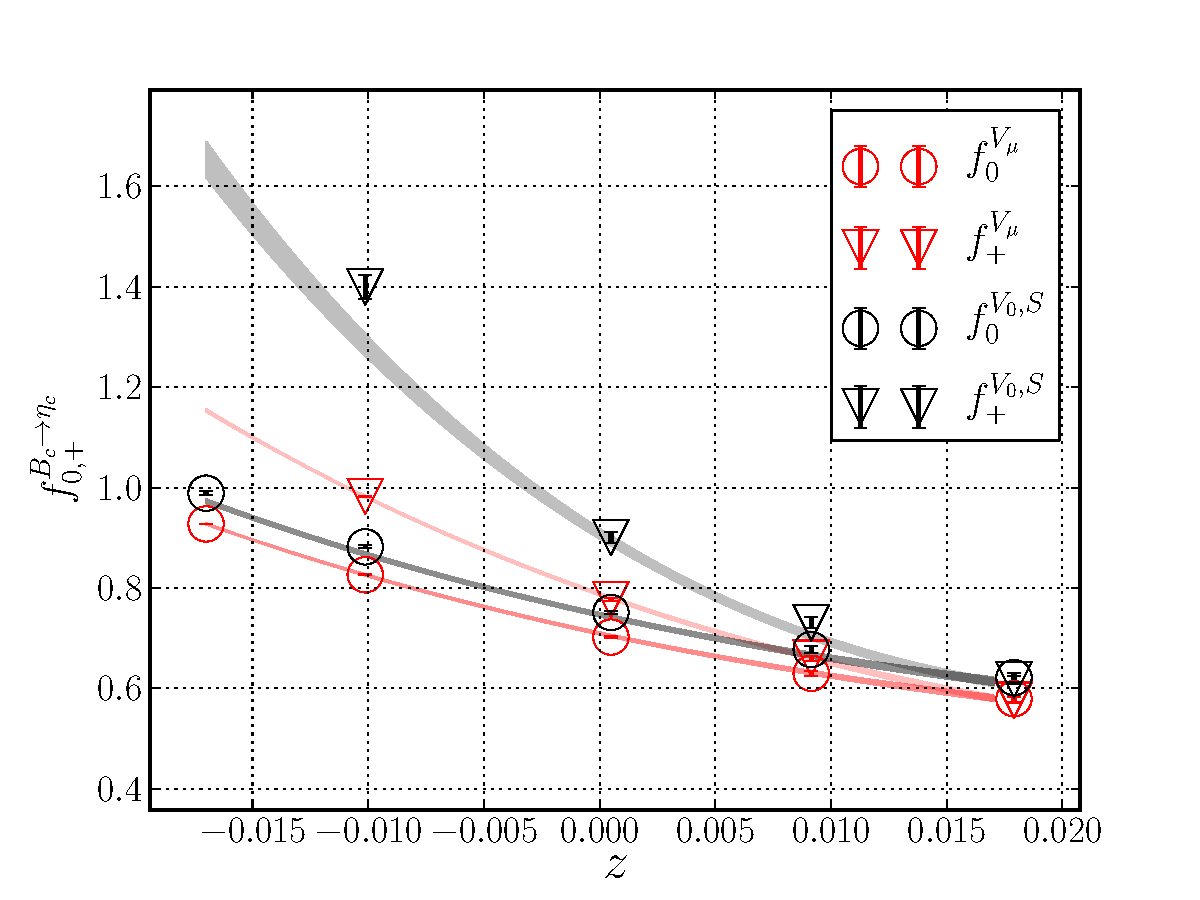
\includegraphics[scale=0.65]{images/NRQCD/Bcetac_bothways_noV0norm.pdf}
\caption{Comparison of form factors from $\langle V_0 \rangle, \langle S \rangle$ and $\langle V_0 \rangle,\langle V_k \rangle$, no additional normalizations.}
\label{fig:naive}
\end{figure}
The divergence is due to the numerator of \eqref{eq:fplus} not tending to zero as ${\textbf{p}}_{\eta_c}^2\to 0$. At ${\textbf{p}}_{\eta_c}^2 = 0$, the numerator becomes $(m_b-m_c) \langle S \rangle - (M_{B_c}-M_{\eta_c}) \langle V_0 \rangle$, which vanishes when the ward identity is satisfied. So one would expect if we renormalize one of the currents so the Ward identity is satisfied (at $q^2_{max}$), this divergence should me removed or at least reduced.
\\ \\
In everything below I'll take the philosophy that we can "trust" the normalization of the scalar current, and use the information in that to renormalize the vector currents. So to satisfy the Ward identity, I multiplied $\langle V_0 \rangle$ by a factor
\begin{align}
	Z_{V_0} = {m_b-m_c \over M_{B_c}-M_{\eta_c} } { \langle S \rangle \over \langle V_0 \rangle }\Big\vert_{q^2_{max}} = 1.0661(36)
	\label{eq:Zward}
\end{align}
This seems to deal with the $f_+$ divergence (fig. \ref{fig:Zward}).
\begin{figure}[htb!]
\centering
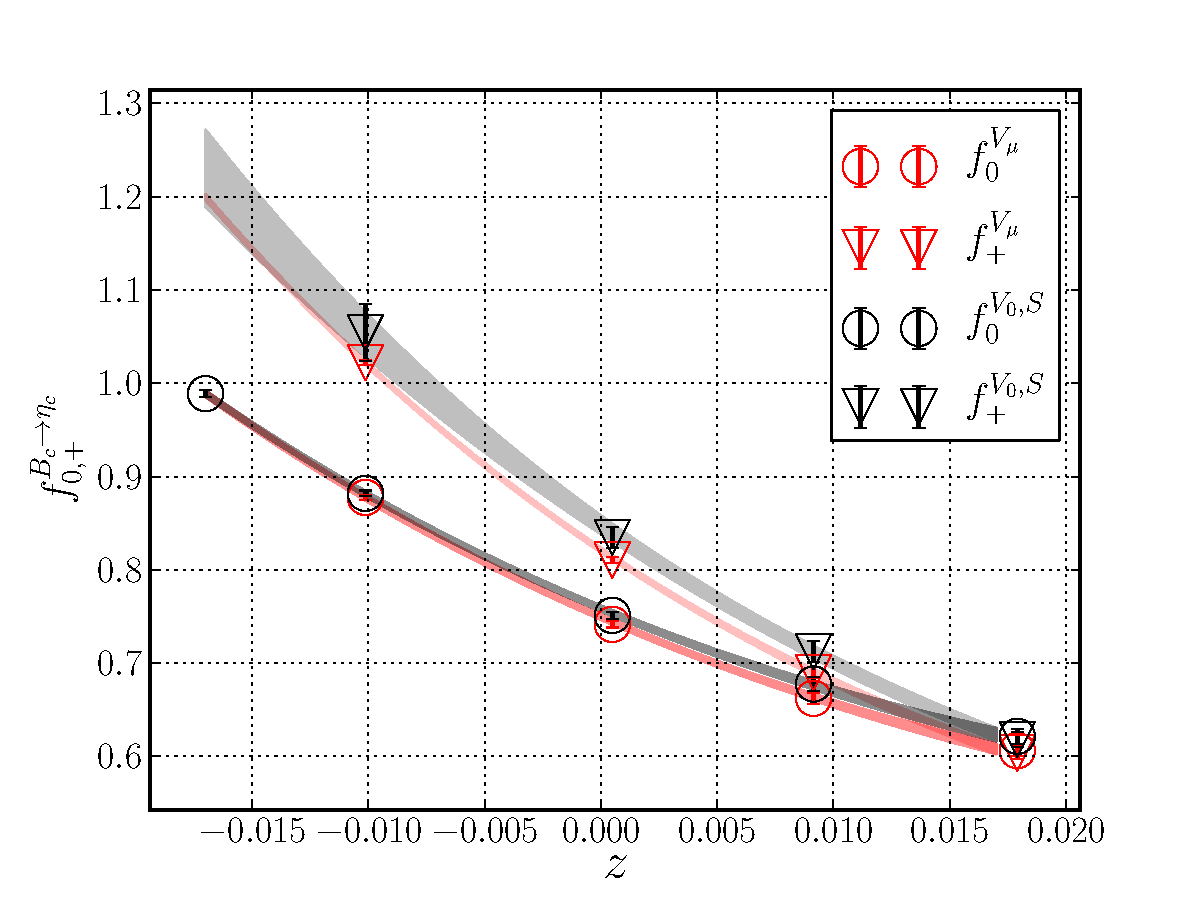
\includegraphics[scale=0.65]{images/NRQCD/Bcetac_bothways.pdf}
\caption{Comparison of form factors from $\langle V_0 \rangle,\langle S \rangle $ and $\langle V_0\rangle,\langle V_k\rangle$, $\langle V_0\rangle$ is mutliplied by $Z_{V_0}$ given in \eqref{eq:Zward}}.
\label{fig:Zward}
\end{figure}
The same technique does not solve the issue in the $B_{(s)}\to D_{(s)}$ case, the divergence is too severe. An alternative could be to find a normalization of $\langle V_k \rangle$ by comparing the two methods on $B_c\to\eta_c$, then get $B_{(s)}\to D_{(s)}$ form factors from $\langle V_0 \rangle, \langle V_k \rangle$, with the renormalized $\langle V_k \rangle$.
\\ \\
We can determine a $Z_{V_k}$ by demanding that $f_{0,+}^{V_0,S}/f_{0,+}^{V_{\mu}}=1$, and claiming that $\langle V_0 \rangle, \langle S \rangle$ require no further normalization. This can be done with both $f_+$ and $f_0$, at any $q^2$. 
\begin{align}
	Z_{V_k} &= 1 + {f_+^{V_0,S} - f_+^{V_{\mu}} \over R_{+k} \langle V_k \rangle }  \\
	&= 1 + {f_0^{V_0,S} - f_0^{V_{\mu}} \over R_{0k} \langle V_k \rangle }
\end{align}
where the $R$'s are some kinematic gunk: $R_{+k} = ( M_{B_c} - E_{\eta_c} )/2M_{B_c}p_{\eta_c}^k$,\\ $R_{0k} = R_{+k} - {( M_{B_c}^2-M_{\eta_c}^2 )(M_{B_c}-E_{\eta_c})/2M_{B_c} p_{\eta_c}^k q^2}$. The form factors here are the ones in fig. \ref{fig:Zward}. The results are shown in fig. \ref{fig:ZVk}.
\begin{figure}[htb!]
\centering
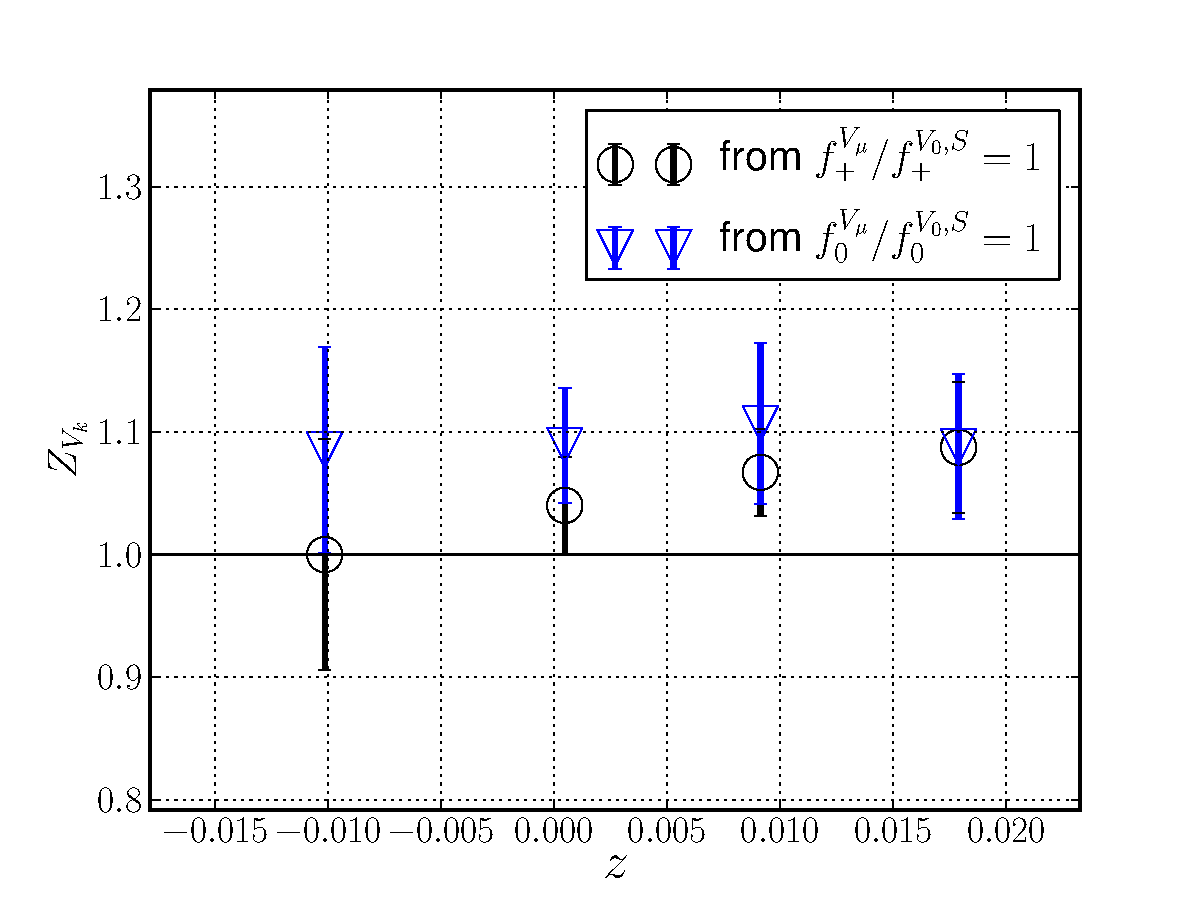
\includegraphics[scale=0.5]{images/NRQCD/ZVk_fromBcetac.pdf}
\caption{$Z_{V_k}$ from constraining form factors to be the same from both methods.}.
\label{fig:ZVk}
\end{figure}
Since these are all estimates of the same value, we can average over them to get
\begin{align}
	Z_{V_k} = 1.070(46)
\end{align}
When this normalization is given to $\langle V_k \rangle$, the $B_c\to\eta_c$ form factors from the two methods become consistent (fig. \ref{fig:identicle})
\begin{figure}[htb!]
\centering
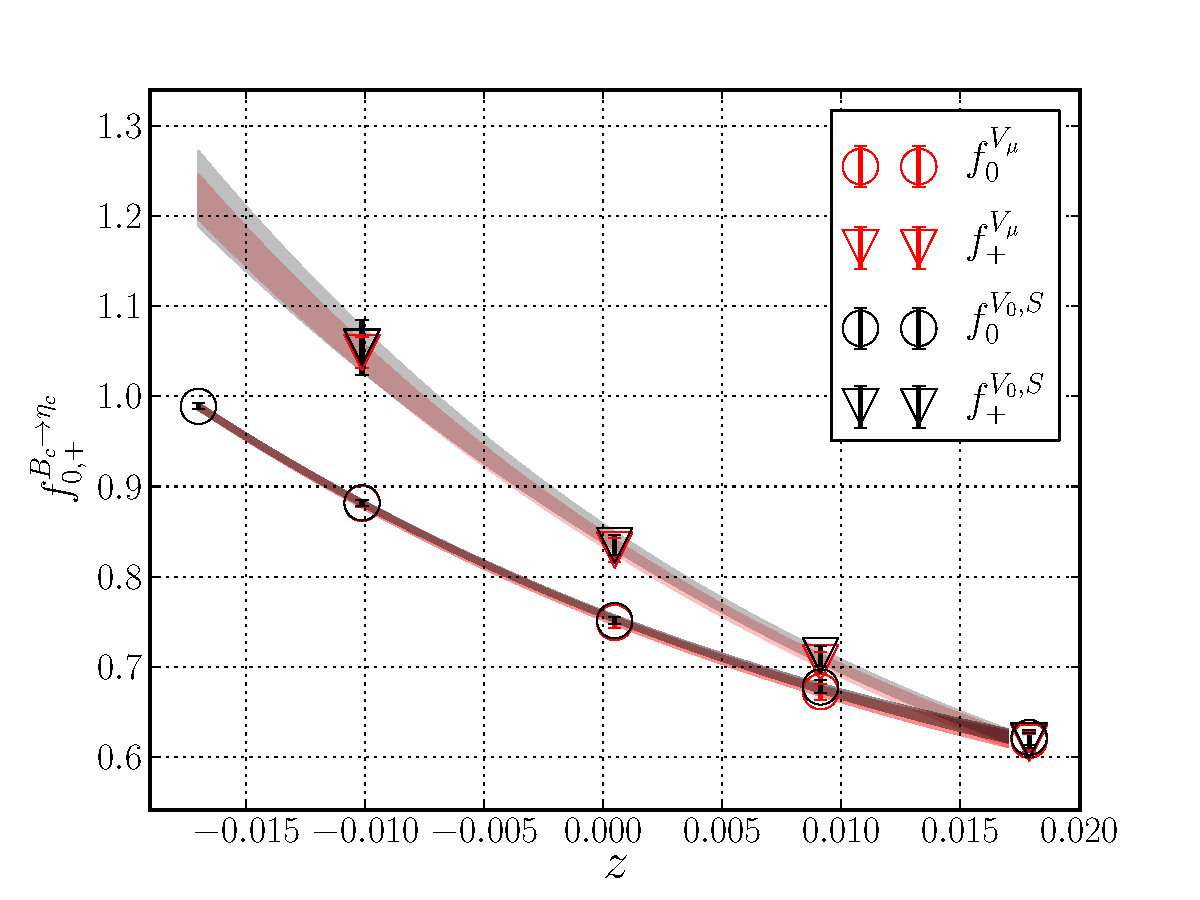
\includegraphics[scale=0.65]{images/NRQCD/Bcetac_bothways_withZVk.pdf}
\caption{Comparison of form factors from $\langle V_0 \rangle, \langle S \rangle$ and $\langle V_0 \rangle,\langle V_k \rangle$, with $\langle V_0 \rangle$ normalized via $Z_{V_0}$ and $\langle V_k \rangle$ normalized with $Z_{V_k}$.}.
\label{fig:ZVk}
\end{figure}
This $Z_{V_k}$ could be slapped onto the $B_{(s)}\to D_{(s)}$ spacial vector current, then we could use that. It has a $4\%$ error, but it's still an improvement on what was happening using $\langle S \rangle$ and $\langle V_0 \rangle$.

\subsection{Another constraint: $f_+$ analyticity}

{\red{
    Are the $z_2$'s for $V_0$ and $S$ not the same? If so, $pf_+$ would have some single extra factor $\propto z_2$, and this could be tuned to force the below condition. Independent determination of $z_2$?
}}

Another thing that could be used to constrain some other normalization is the condition that the numerator of $f_+$ tends towards zero as ${\textbf{p}}^2_{\eta_c}\to 0$:
\begin{align}
	\displaystyle{\lim_{{\textbf{p}}_{\eta_c}^2\to 0}}\quad {1\over2M_{B_c}}\big( \delta^M  \langle S \rangle - q^2 \langle V_0 \rangle \big) = \displaystyle{\lim_{{\textbf{p}}_{\eta_c}^2\to 0}} \quad {\textbf{p}}^2_{\eta_c}f_+ = 0
\end{align}
This is not guaranteed even when $\langle V_0 \rangle$ is normalized to satisfy the Ward identity. In fig. \ref{fig:p2fp}, all the $q^2\neq q^2_{max}$ data is extrapolated to $q^2_{max}$, with fit form
\begin{align}
	{\textbf{p}}^2_{\eta_c}f_+ = r + {{\textbf{p}}^2_{\eta_c} \over P(q^2)}\sum a^+_n z^n
\end{align}
i.e., the usual z-expansion, with an extra fit parameter $r$ which represents the residue of $f_+$ at $q^2_{max}$ if one trusts the $q^2\neq q^2_{max}$ data.

\begin{figure}[htb!]
\centering
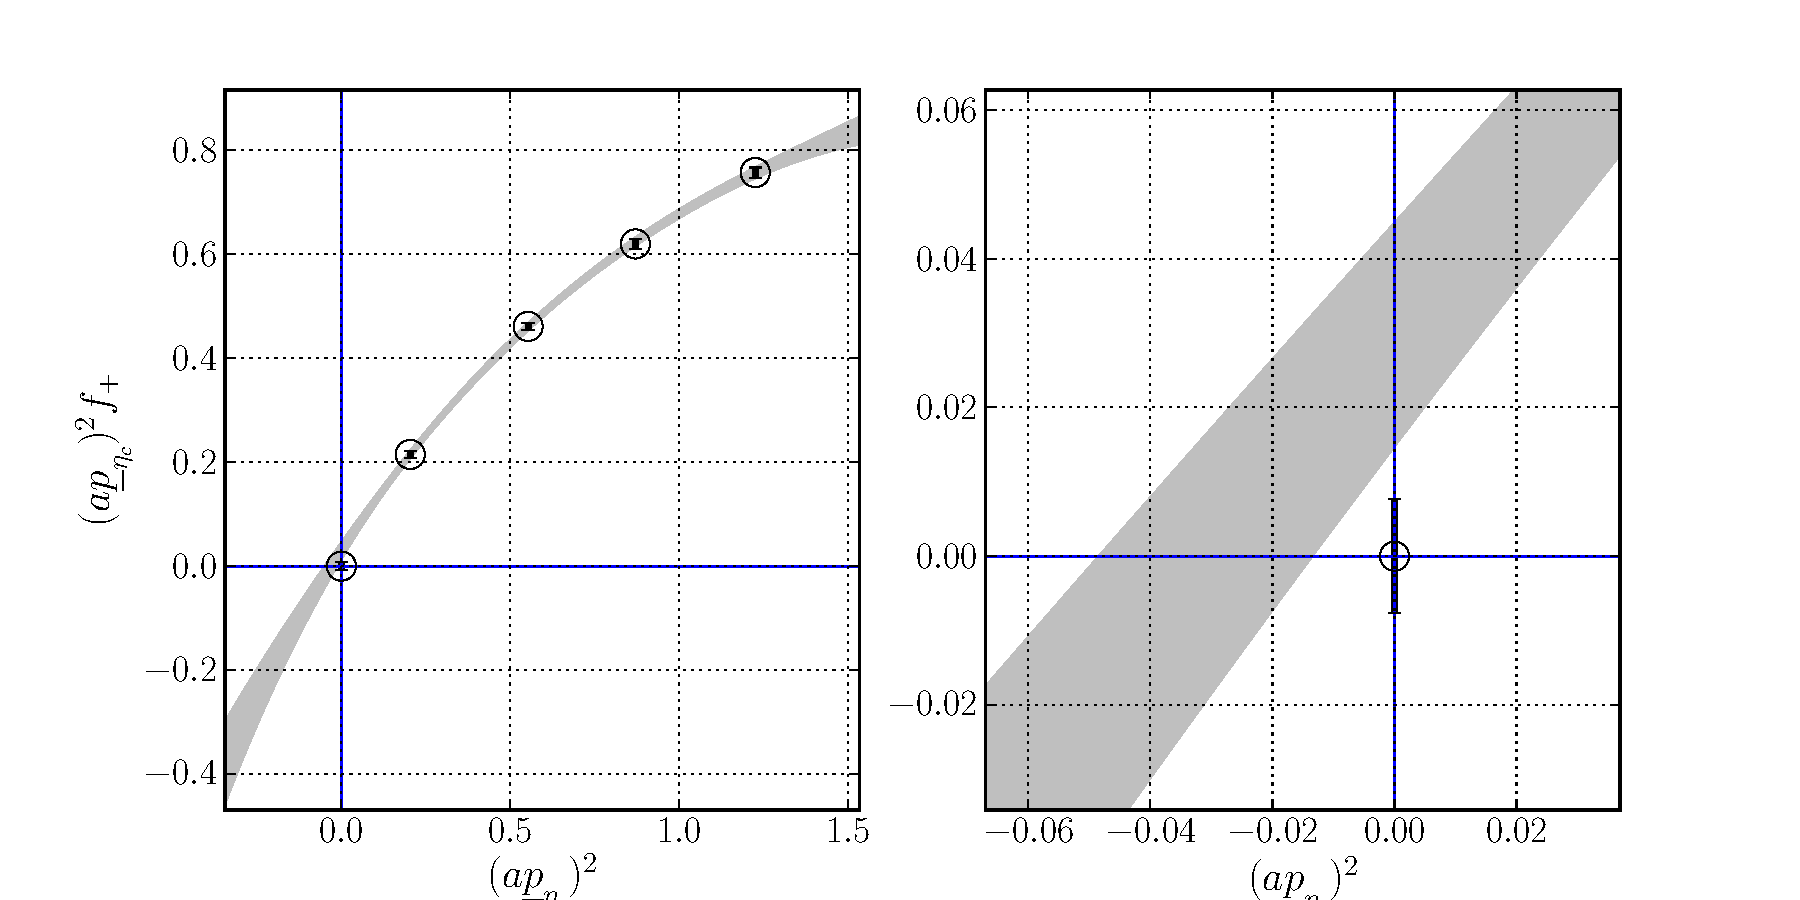
\includegraphics[scale=0.45]{images/NRQCD/p2fp_Bcetac_ward.pdf}
\caption{\label{fig:p2fp}.}
\end{figure}
This fit results in a residue of $r = 0.030(15)$. Perhaps there's something that can be normalized by demanding that $r=0(0)$. I haven't worked out a good way to implement this though, and where that information should go.

